\chapter{Elenco delle primitive}

\label{liste-prim} La tartaruga è comandata tramite comandi interni chiamati \emph{`primitive'}. Le seguenti sezioni descrivono le primitive di \xlogo.


\section{Movimento della tartaruga, impostazioni del tratto e del colore}
\subsection{Movimento}
Queste prime primitive governano il movimento della tartaruga.\\

\prim{Avanti, Av}{n}
 Sposta la tartaruga in avanti di n passi, nella direzione in cui si trova.\\

\prim{Indietro, In}{n}
 Sposta la tartaruga indietro di n passi, nella direzione in cui si trova.\\

\prim{RuotaDestra, DX}{n}
 Ruota la tartaruga di n gradi verso la sua destra (rispetto la direzione in cui si trova).\\

\prim{RuotaSinistra, SX}{n}
 Ruota la tartaruga di n gradi verso la sua sinistra (rispetto la direzione in cui si trova).\\

\prim{Cerchio, Circonferenza}{R}
 Disegna una circonferenza di raggio R avente come centro la tartaruga.\\

\prim{Arco}{R ang1 ang2}
 Disegna una arco di circonferenza di raggio R attorno alla tartaruga. L'arco è viene tracciato dall'angolo ang1 all'angolo ang2.\\

\prim{Origine}{}
 Riporta la tartaruga alla sua posizione iniziale ossia alle coordinate {[}0 0{]} con direzione 0 gradi.\\

\prim{ImpostaPosizione, ImpPos}{elenco}
 Sposta la tartaruga alle coordinate x e y specificate nell'elenco (x si riferisce all'asse delle x, y all'asse delle y).\\
 Esempio: \texttt{ImpPos [50 30]}\\

\prim{ImpostaX, ImpX}{x}
 Sposta la tartaruga orizzontalmente fino al punto x sull'asse delle ascisse (X).\\

\prim{ImpostaY, ImpY}{y}
 Sposta la tartaruga verticalmente fino al punto y sull'asse delle ordinate (Y).\\

\prim{ImpostaXY, ImpXY}{x y}
 Identico a \texttt{ImpPos {[}x y{]}}\\

\prim{ImpostaDirezione, ImpDir}{n}
 Orienta la tartaruga nelle direzione n (0-360 gradi), dove 0 corrisponde alla direzione verticale verso l'alto (Nord), 90 alla direzione orizzontale verso destra (Est) e così via in base all'orientamento della bussola. \\

\prim{Etichetta}{arg}
 Disegna arg a partire dalla posizione della tartaruga, ruotato di 90 gradi verso destra. arg può essere una parola od un elenco.\\
 Esempio: \texttt{Etichetta [Ciao lì fuori!]} scriverà la frase ``''Ciao lì fuori!'' ovunque la tartaruga sia, in direzione orizzontale.\\
 Esempio: \texttt{SX 90} \texttt{Etichetta [Ciao lì fuori!]} scriverà la frase ``Ciao lì fuori!" ovunque la tartaruga sia, in direzione verticale verso l'alto.\\

\prim{Punto}{elenco}
 Illumina nel colore della penna il punto identificato dalle coordinate nell'elenco.\\
Esempio: \texttt{Punto [100 50]} Illumina il punto di coordinate x 100 e y 50.\\
\subsection{Proprietà della tartaruga}
In questo secondo gruppo rientrano le primitive che impostano le proprietà della tartaruga. Per esempio la tartaruga è visibile sullo schermo? Di che colore dovrebbe essere il tratto quando si sposta? \\

\prim{MostraTartaruga, MT}{}
 Rende visibile la tartaruga sullo schermo.\\

\prim{NascondiTartaruga, NT}{}
 Rende la tartaruga invisibile sullo schermo.\\

\prim{PulisciSchermo, PSc}{}
 Svuota l'area di disegno.\\

\prim{Pulisci}{}
 Svuota l'area di disegno ma lascia la tartaruga nello stesso posto.\\

\prim{ResettaTutto, InizializzaTutto}{}
 Riporta l'interfaccia di \xlogo\ ai valori iniziali e svuota l'area di disegno. I valori iniziali sono:
\begin{itemize}
	\item Colore della penna: nero
	\item Forma della penna: quadrata
	\item Qualità del tratto: normale
	\item Colore dello schermo: bianco
	\item Dimensioni dello schermo: 1000x1000
	\item Modalità animazione: disabilitata
	\item Font del testo e della grafica: Dialog 12 punti
	\item Numero tartarughe ammesse: 16
	\item Modalità traccia: disabilitata
\end{itemize}

\prim{PennaGiu, PennaGiu, PG}{}
 Quando la penna è abbassata la tartaruga traccia il percorso che compie mentre si sposta.\\

\prim{PennaSu, PennaSu, PS}{}
 Quando la penna è alzata la tartaruga si sposta senza tracciare il proprio percorso.\\

\prim{CancellaPenna, CP}{}
 La tartaruga cancella qualsiasi segno incontro al proprio passaggio.\\

\prim{InvertiPenna, InvPenna}{}
 Abbassa la penna e pone la tartaruga in modalità inversa.\\

\prim{PennaDisegno, PD}{}
 Abbassa la penna e pone la tartaruga nella modalità classica di disegno.\\

\prim{ImpostaColorePenna, ImpCP}{colore}
 Imposta il colore della penna, cfr. pagina \pageref{couleurs} per l'elenco dei colori.\\

\prim{ImpostaColoreSfondo, ImpCS}{colore}
 Imposta il colore dello sfondo, cfr. pagina \pageref{couleurs} per l'elenco dei colori.\\

\prim{Posizione, Pos}{}
 Restituisce la posizione attuale della tartaruga.\\
Esempio: \texttt{Pos} ritorna {[}10 -100{]}\\

\prim{x}{}
 Restituisce la coordinata X della posizione della tartaruga.\\

\prim{y}{}
 Restituisce la coordinata Y della posizione della tartaruga.\\

\prim{z}{}
 Restituisce la coordinata Z della posizione della tartaruga (Disponibile solamente nella modalità 3D).\\

\prim{Direzione}{}
 Restituisce la direzione in gradi della tartaruga (cfr. \texttt{ImpostaDirezione})  \\
\prim{Verso}{elenco}
 Restituisce la direzione verso cui la tartaruga dovrebbe puntare per raggiungere il punto definito dalle coordinate definite in \textit{elenco}. Elenco deve contenere due numeri che rappresentino le coordinate x e y del punto.\\
\prim{Distanza}{elenco}
Restituisce il numero di passi che la tartaruga dovrebbe compiere per raggiungere il punto definito dalle coordinate definite in \textit{elenco}. Elenco deve contenere due numeri che rappresentino le coordinate x e y del punto.\\
\prim{ColorePenna, ColP}{}
 Restituisce il colore della penna attuale. Il colore è definito come un elenco di tre numeri [r g b] dove r è la componente rossa, b è la componente blu, g è la componente verde.  \\
\prim{ColoreSfondo, ColS}{}
 Restituisce il colore dello sfondo attuale. Il colore è definito come un elenco di tre numeri [r g b] dove r è la componente rossa, b è la componente blu, g è la componente verde.  \\
\prim{Finestra}{}
 Si permette alla tartaruga di muoversi fuori dalla area di disegno (senza disegnarci, ovviamente).\\
\prim{Gira}{}
 Si permette alla tartaruga di lasciare l'area di disegno e riapparire dal lato opposto!\\
\prim{Recinta}{}
 Non si permette alla tartaruga di lasciare l'area di disegno. Nel momento in cui sta per uscirne comparirà un messaggio di errore che informerà del numero massimo di passi che la tartaruga può compiere prima di raggiungere il punto di uscita.\\
\prim{Prospettiva, 3D}{}
 La tartaruga può spostarsi in uno spazio a 3 dimensioni (cfr. la sezione speciale \ref{3D} per questa modalità). Per tornare alla modalità classica 2D, utilizzare una delle 3 primitive \texttt{Finestra}, \texttt{Gira} or \texttt{Recinta}\\
\prim{CercaColore, CC}{elenco}
 Restituisce il colore del punto nell'area di disegno identificato dalle coordinate x e y fornite in elenco \textit{elenco}. Il colore è definito come un elenco di tre numeri [r g b] dove r è la componente rossa, b è la componente blu, g è la componente verde.\\
\prim{ImpSpessorePenna, ImpSP}{n}
 Imposta lo spessore della penna della tartaruga in pixel (o passi). Lo spessore iniziale è 1. La penna ha una forma quadrata o rotonda (altre forme saranno introdotte in versioni future di \xlogo).\\
\prim{SpessorePenna, SP}{}
 Restituisce lo spessore nella penna della tartaruga in punti (o passi).\\
\prim{ImpFormaPenna, ImpFP}{0-1}
 Imposta la forma della penna, quadrata o rotonda:
\begin{itemize}
	\item 0$\to$quadrata.
	\item 1$\to$rotonda.
\end{itemize}
\noindent
\prim{FormaPenna, FP}{}
Restituisce la forma della penna.
\begin{itemize}
	\item 0$\to$quadrata.
	\item 1$\to$rotonda.
\end{itemize}
\noindent
\prim{ImpQualitaDisegno, ImpQD}{0-1-2}
Imposta la qualità del disegno :
\begin{itemize}
	\item  0$\to$normale.
	\item  1$\to$alta.
	\item  2$\to$bassa.
\end{itemize}
\noindent
\prim{QualitaDisegno, QD}{}
Restituisce la qualità del disegno.
\begin{itemize}
	\item  0$\to$normale.
	\item  1$\to$alta.
	\item  2$\to$bassa.
\end{itemize}
\noindent
\prim{ImpDimensioneSchermo}{elenco}
Imposta la dimensione dell'area di disegno ai valori x e y definiti in \textit{elenco}. \texttt{ImpDimensioneSchermo [1000 1000]}\\
\prim{DimensioneSchermo}{}
Restituisce un elenco di due numeri con la dimensioni dell'area di disegno.\\
\prim{ImpostaForma, ImpFo}{n}
Si può scegliere la forma della tartaruga nel secondo tab della finestra aperta da Opzioni-Preferenze... Ma si può impostare la tartaruga preferita con \texttt{ImpostaForma}. Il numero \textit{n} varia da 0 a 6 (0 rappresenta la forma triangolare).\\
\prim{Forma}{}
Restituisce il numero che rappresenta la forma della tartaruga.\\
\prim{ImpostaCorpoFont, ImpCFont}{n}
Quando si scrive nell'area di disegno con la primitiva \texttt{Etichetta}, si può modificare il corpo (ossia le dimensioni) del font iniziale che è 12.\\
\prim{CorpoFont}{}
Restituisce il corpo (le dimensioni) del font impostato per quando si scrive nell'area di disegno con la primitiva  \texttt{Etichetta}.\\
\prim{ImpostaNomeFont, ImpNFont}{n}
Imposta il numero $n$ del font quando si scrive nell'area di disegno con la primitiva \texttt{Etichetta}. L'elenco dei font ed i relativi numeri $n$ da utilizzare si trova nel Tab \textit{Font} del menu Strumenti$\to$Preferenze.\\
\prim{ImpostaAllineamentoTesto, ImpAllTesto}{elenco}
Imposta l'allineamento attorno alla tartaruga da utilizzare quando si scrive nell'area di disegno con la primitiva \texttt{Etichetta}. \textit{elenco} contiene due numeri interi.
\begin{itemize}
 \item Il primo numero si riferisce all'allineamento orizzontale:
	\begin{itemize}
 	\item 0: allineamento a sinistra
	\item 1: allineamento al centro
	\item 2: allineamento a destra
	\end{itemize}
 \item Il secondo numero si riferisce all'allineamento verticale:
	\begin{itemize}
 	\item 0: allineamento in basso
	\item 1: allineamento al centro
	\item 2: allineamento in alto
	\end{itemize}
\end{itemize}
Tutti i possibili casi che si possono verificare sono di seguito elencati.
\texttt{ImpCFont 50 Etichetta "XLogo}
\begin{center}
	\begin{tabular}{|c|c|c|}
		\hline
		
\includegraphics[width=3cm]{pics/fap20.png} & 
\includegraphics[width=3cm]{pics/fap10.png} & 
\includegraphics[width=3cm]{pics/fap00.png} \\
		\texttt{ImpAllTesto [2 0]} & \texttt{ImpAllTesto [1 0]} & \texttt{ImpAllTesto [0 0]}\\
		\hline
		
\includegraphics[width=3cm]{pics/fap21.png}& 
\includegraphics[width=3cm]{pics/fap11.png} & 
\includegraphics[width=3cm]{pics/fap01.png} \\
		\texttt{ImpAllTesto [2 1]} & \texttt{ImpAllTesto [1 1]} & \texttt{ImpAllTesto [0 1]}\\
		\hline
		
\includegraphics[width=3cm]{pics/fap22.png}& 
\includegraphics[width=3cm]{pics/fap12.png} & 
\includegraphics[width=3cm]{pics/fap02.png} \\
		\texttt{ImpAllTesto [2 2]} & \texttt{ImpAllTesto [1 2]} & \texttt{ImpAllTesto [0 2]}\\
		\hline
	\end{tabular}
\end{center}
\hspace{0cm}\\
\prim{AllineamentoTesto}{}
 Restituisce un elenco di due elementi che rappresenta l'allineamento del testo attorno alla tartaruga, quando si utilizza \texttt{Etichetta} per scrivere nell'area di disegno.\\
\prim{NomeFont, NF}{}
 Restituisce un elenco di due elementi. Il primo è il numero corrispondente al font utilizzato da \texttt{Etichetta}. Il secondo elemento è un elenco che contiene il nome del font.\\
\prim{ImpostaSeparazione,ImpSep}{n}
 Determina il rapporto tra l'area di disegno e l'area dello storico dei comandi. Il numero $n$ deve essere incluso tra 0 e 1. Quando $n$ è uguale a 1 l'intera area è occupata dall'area di disegno, quando $n$ è uguale a 0 l'area con lo storico dei comandi usa tutto lo spazio.\\
\prim{Separazione,Sep}{}
 Restituisce il rapporto attuale tra l'area di disegno e l'area con lo storico dei comandi.\\
\prim{Griglia}{a b}
 Disegna una griglia, con ciascun rettangolo avente dimensioni $a$ e $b$.\\
\prim{CancellaGriglia,CancGriglia}{}
 Elimina la griglia eventualmente disegnata.\\
\prim{ImpostaColoreGriglia,ImpColGriglia}{colore}
 Permette di impostare il colore desiderato per la griglia. Il colore è definito come un elenco di tre numeri [r g b] dove r è la componente rossa, b è la componente blu, g è la componente verde.\\
\prim{ColoreGriglia}{}
 Restituisce il colore della griglia attuale.\\
\prim{Griglia?}{}
 Restituisce vero se la griglia è disegnata, altrimenti restituisce falso.\\
\prim{Assi}{n}
 Disegna gli assi orizzontale e verticale. La distanza tra due divisioni è $n$ passi. \\
\prim{AsseX}{n}
 Disegna l'asse orizzontale. La distanza tra due divisioni è $n$ passi.\\
\prim{AsseY}{n}
 Disegna l'asse verticale. La distanza tra due divisioni è $n$ passi.\\
\prim{CancellaAssi,CancAssi}{}
 Cancella entrambi gli assi.\\
\prim{ImpostaColoreAssi, ImpColAssi}{colore}
 Imposta il colore con cui disegnare gli assi. Il colore è definito come un elenco di tre numeri [r g b] dove r è la componente rossa, b è la componente blu, g è la componente verde. \\
\prim{ColoreAssi}{}
 Restituisce il colore attuale degli assi.\\
\prim{AsseX?}{}
 Restituisce vero se l'asse orizzontale è disegnato, altrimenti restituisce falso.\\
\prim{AsseY?}{}
 Restituisce vero se l'asse verticale è disegnato, altrimenti restituisce falso.\\
\prim{ImpostaZoom,ImpZoom}{a}
 Ingrandisce l'area di disegno di un fattore $a$ che rappresenta la scala rispetto alle dimensioni originali dell'immagine definite nel pannello delle preferenze.\\
\prim{Zoom}{}
 Restituisce l'attuale scala di zoom.\\
\prim{LunghezzaEtichetta,LE}{arg}
 Restituisce la lunghezza del testo da scrivere nell'area di disegno con la primitiva \texttt{Etichetta}, utilizzando il font attuale. \\
\prim{DimensioneZona}{}
 Retituisce un elenco che contiene quattro numeri interi. L'elenco rappresenta le coordinate dell'angolo sinistro in alto e le coordinate dell'angolo destro in basso.\\
\prim{Messaggio, msg}{elenco}
 Visualizza una finestra di dialogo con il messaggio in \textit{elenco}. L'esecuzione del programma viene fermata fino a ché l'utente clicca il bottone ``OK''.\\
\subsection{Qualche parola sui colori}
 I colori sono definiti in \xlogo\ come un elenco di tre numeri \texttt{[r g b]}, ciascuno compreso tra 0 e 255,  dove r è la componente rossa, b è la componente blu, g è la componente verde. \xlogo\ ha 16 colori predefiniti i quali possono essere richiamati con il loro elenco rgb o con una primitiva: \label{couleurs}
\begin{center}
\begin{longtable}{*{4}{|c}|}
\hline
Numeri & Primitive & [R G B] & Color \\ \endhead
\hline
0& \texttt{Nero} & [0 0 0] & \index{Nero}
\begin{minipage}[m]{1.5cm}
\begin{center}
\vspace{0.2cm}

\includegraphics[width=1 cm]{pics/couleur0.png}
\vspace{0.2cm}
\end{center}
\end{minipage}\\
\hline
1 & \texttt{Rosso} & [255 0 0] & \index{Rosso}
\begin{minipage}[m]{1.5cm}
\begin{center}
\vspace{0.2cm}

\includegraphics[width=1 cm]{pics/couleur1.png}
\vspace{0.2cm}
\end{center}
\end{minipage}\\\hline
2 & \texttt{Verde} & [0 255 0] & \index{Verde}
\begin{minipage}[m]{1.5cm}
\begin{center}
\vspace{0.2cm}

\includegraphics[width=1 cm]{pics/couleur2.png}
\vspace{0.2cm}
\end{center}
\end{minipage}\\
\hline
3 & \texttt{Giallo} & [255 255 0] & \index{Giallo}
\begin{minipage}[m]{1.5cm}
\begin{center}
\vspace{0.2cm}

\includegraphics[width=1 cm]{pics/couleur3.png}
\vspace{0.2cm}
\end{center}
\end{minipage}\\
\hline
4 & \texttt{Blu} & [0 0 255] & \index{Blu}
\begin{minipage}[m]{1.5cm}
\begin{center}
\vspace{0.2cm}

\includegraphics[width=1 cm]{pics/couleur4.png}
\vspace{0.2cm}
\end{center}
\end{minipage}\\
\hline
5 & \texttt{Magenta} & [255 0 255] & \index{Magenta}
\begin{minipage}[m]{1.5cm}
\begin{center}
\vspace{0.2cm}

\includegraphics[width=1 cm]{pics/couleur5.png}
\vspace{0.2cm}
\end{center}
\end{minipage}\\
\hline
6 & \texttt{Ciano} & [0 255 255] & \index{Ciano}
\begin{minipage}[m]{1.5cm}
\begin{center}
\vspace{0.2cm}

\includegraphics[width=1 cm]{pics/couleur6.png}
\vspace{0.2cm}
\end{center}
\end{minipage}\\
\hline
7 & \texttt{Bianco} & [255 255 255] & \index{Bianco}
\begin{minipage}[m]{1.5cm}
\begin{center}
\vspace{0.2cm}

\includegraphics[width=1 cm]{pics/couleur7.png}
\vspace{0.2cm}
\end{center}
\end{minipage}\\
\hline
8 & \texttt{Grigio} & [128 128 128] & \index{Grigio}
\begin{minipage}[m]{1.5cm}
\begin{center}
\vspace{0.2cm}

\includegraphics[width=1 cm]{pics/couleur8.png}
\vspace{0.2cm}
\end{center}
\end{minipage}\\
\hline
9 & \texttt{GrigioChiaro} & [192 192 192] & \index{GrigioChiaro}
\begin{minipage}[m]{1.5cm}
\begin{center}
\vspace{0.2cm}

\includegraphics[width=1 cm]{pics/couleur9.png}
\vspace{0.2cm}
\end{center}
\end{minipage}\\
\hline
10 & \texttt{RossoScuro} & [128 0 0] & \index{RossoScuro}
\begin{minipage}[m]{1.5cm}
\begin{center}
\vspace{0.2cm}

\includegraphics[width=1 cm]{pics/couleur10.png}
\vspace{0.2cm}
\end{center}
\end{minipage}\\
\hline
11 & \texttt{GrigioScuro} & [0 128 0] & \index{GrigioScuro}
\begin{minipage}[m]{1.5cm}
\begin{center}
\vspace{0.2cm}

\includegraphics[width=1 cm]{pics/couleur11.png}
\vspace{0.2cm}
\end{center}
\end{minipage}\\
\hline
12 & \texttt{BluScuro} & [0 0 128] & \index{BluScuro}
\begin{minipage}[m]{1.5cm}
\begin{center}
\vspace{0.2cm}

\includegraphics[width=1 cm]{pics/couleur12.png}
\vspace{0.2cm}
\end{center}
\end{minipage}\\
\hline
13 & \texttt{Arancio} & [255 200 0]& \index{Arancio}
\begin{minipage}[m]{1.5cm}
\begin{center}
\vspace{0.2cm}

\includegraphics[width=1 cm]{pics/couleur13.png}
\vspace{0.2cm}
\end{center}
\end{minipage}\\
\hline
14 & \texttt{Rosa} & [255 175 175] & \index{Rosa}
\begin{minipage}[m]{1.5cm}
\begin{center}
\vspace{0.2cm}

\includegraphics[width=1 cm]{pics/couleur14.png}
\vspace{0.2cm}
\end{center}
\end{minipage}\\
\hline
15 & \texttt{Violetto} & [128 0 255] & \index{Violetto}
\begin{minipage}[m]{1.5cm}
\begin{center}
\vspace{0.2cm}

\includegraphics[width=1 cm]{pics/couleur15.png}
\vspace{0.2cm}
\end{center}
\end{minipage}\\
\hline
16 & \texttt{Marrone} & [153 102 0] & \index{Marrone}
\begin{minipage}[m]{1.5cm}
\begin{center}
\vspace{0.2cm}

\includegraphics[width=1 cm]{pics/couleur16.png}
\vspace{0.2cm}
\end{center}
\end{minipage}\\
\hline
\end{longtable} 
\end{center}
\begin{lstlisting}[caption="Tre istruzioni identiche per impostare il colore dello schermo"]
ImpCS Arancio
ImpCS 13
ImpCS [255 200 0]
\end{lstlisting}


\subsection{Modalità Animazione}
Le seguenti sono tre primitive che consentono l'esecuzione dei comandi in modo più veloce del solito. La tartaruga non si muoverà più fino a che non le viene imposto di ridisegnare lo schermo mediante la primitiva \textit{Aggiorna}. Il vantaggio della modalità Animazione consiste nella maggiore velocità di disegno che consente di creare animazioni.\\
\prim{Animazione}{}
 La tartaruga entra nella modalità Animazione. Da questo momento non verrà disegnato niente sullo schermo se non quando si utilizza la primitiva \texttt{Aggiorna}.\\
\prim{FermaAnimazione}{}
 La tartaruga esce dalla modalità Animazione.\\
\prim{Aggiorna,Ridisegna}{}
 In modalità Animazione aggiorna l'area di disegno per riflettere tutte le primitive eseguite dal momento dell'ingresso nella modalità.\\ \\
 Per identificare la modalità Animazione, una icona con una telecamera appare nella finestra dello storico dei comandi. Se l'icona viene cliccata si esce dalla modalità.
\begin{center}
   
\includegraphics[scale=2.5]{pics/animation.png}
\end{center} 

\subsection{Scrivere nell'area di testo con le primitive \texttt{Stampa} e \texttt{Scrivi}}

La seguente tabella espone le primitive che permettono di modificare le proprietà dell'area di testo. Le primitive che controllano il colore e le dimensioni dell'area dello storico dei comandi influenzano solo le primitive  \texttt{Stampa} o \texttt{Scrivi}\\
\prim{PulisciTesto, PT}{}
Svuota l'area dello storico dei comandi.\\
\prim{Stampa, St}{arg}
Scrive l'argomento \textit{arg} nell'area dello storico dei comandi.
\begin{lstlisting}[caption="La primitiva \texttt{Stampa}"]
Stampa "abcd # abcd
St [1 2 3 4] #1 2 3 4
St 4 # 4
\end{lstlisting}
\noindent \prim{Scrivi}{arg1}
Come la primitiva \texttt{Stampa} scrive \textit{arg1} nell'area dello storico dei comandi ma senza andare a capo.\\
 \prim{ImpostaDTesto, ImpDT}{n}
 Imposta il corpo del font nell'area dello storico dei comandi. Disponibile solo per la primitiva \texttt{Stampa}\\
\prim{DimensioneTesto, DT}{}
 Restituisce il corpo del font per la primitiva \texttt{Stampa}.\\
\prim{ImpostaColoreTesto, ImpCT}{colore}
Imposta il colore del font nell'area dello storico dei comandi. Disponibile solo per la primitiva \index{Stampa}. Confronta pag. \pageref{couleurs}.\\
\prim{ColoreTest, CT}{}
 Restituisce il colore del font nell'area dello storico dei comandi.\\
\prim{ImpostaNomeTesto, ImpNTesto}{n}
 Seleziona il font numero \textit{n} per la scrittura con la primitiva \texttt{Stampa} nell'area dello storico dei comandi. Il collegamento tra il font ed il suo numero si può trovare nel Menu$\to$Strumenti$\to$Preferenze$\to$Tab Font.\\
\prim{NomeTesto, NT}{}
Restituisce il font utilizzato nell'area dello storico dei comandi sotto forma di lista. Il primo elemento della lista corrisponde al numero del font utilizzato, il secondo elemento è una lista che riporta il nome del font stesso.\\
\prim{ImpostaStile, ImpSt}{arg}
Imposta il formato del testo nell'area dello storico dei comandi. Si può scegliere tra \texttt{Nessuno, Grassetto, Corsivo, Barrato, Sottolineato, Apice, Pedice}. Per impostare più stili contemporaneamente raggrupparli in un elenco.\\
Alcuni esempi:\\ \\
\texttt{ImpostaStile [Grassetto Sottolineato] Stampa \textquotedbl Ciao}\\
\textbf{\underline{Ciao}}\\
\texttt{ImpSt \textquotedbl Barrato Scrivi [Barrato] ImpSt \textquotedbl Corsivo Scrivi \textquotedbl \textbackslash x ImpSt \textquotedbl Apice Stampa 2}\\
\sout{Barrato} $x^2$\\
\prim{Stile, st}{}
Restituisce un elenco contenente i diversi stili utilizzati per la primitiva \texttt{Stampa}.



\section{Operazioni matematiche}

\prim{Somma}{x y}
 Addiziona i due numeri $x$ e $y$ e ne restituisce il risultato.\\
 Esempio: \texttt{Somma} \ 40 60 restituisce 100\\
\prim{Differenza}{x y}
 Restituisce $x-y$.\\
 Esempio: \texttt{Differenza} \ 100 20 restituisce 80\\
\prim{Meno}{x}
 Restituisce il negativo di $x$. \\
Esempio: \texttt{Meno} \ 5 restituisce -5. \emph{Leggere la nota alla fine del paragrafo.}\\
\prim{Prodotto}{x y}
 Restituisce il risultato della moltiplicazione di $x$ per $y$.\\
\prim{Div, Dividi}{x y}
 Restituisce il risultato della divisione di $x$ per $y$\\
 Esempio: \texttt{Div} \ 3 6 restituisce 0.5\\
\prim{Quoziente}{x y}
Restituisce il quoziente della divisione di $x$ per $y$\\
 \texttt{Quoziente} \ 15 6 restituisce 2\\
\prim{Resto}{x y}
 Restituisce il resto della divisione di $x$ per $y$.\\
\prim{mod, modulo}{x y}
 Restituisce $x$ modulo $y$. 
La seguente tabella dimostra la differenza tra \texttt{modulo x y } e \texttt{Resto x y}.\\
\begin{center}
	$\begin{array}{|c|c|c|c|}
	\hline
	x & y & \textrm{\texttt{Resto x y}} & \textrm{\texttt{modulo x y}} \\
	\hline
	14 & 5 & 4& 4\\
	\hline
	-14 & 5 &-4 & 1\\
	\hline
	14 & -5 & 4 & -1\\
	\hline
	-14 & -5 & -4 & -4 \\
	\hline
\end{array}
$
\end{center}
\prim{Arrotonda}{x}
Restituisce il più vicino numero intero a $x$.\\
\begin{center}
$\begin{array}{|c|c|}
	\hline \textrm{Istruzione} & \textrm{Risultato} \\ \hline
	\texttt{Arrotonda 8.9} 		& \texttt{9}\\
	\hline
	\texttt{Arrotonda 6.8} 		& \texttt{7} \\
	\hline
	\texttt{Arrotonda 6.2} 		& \texttt{6} \\
	\hline
\end{array}$
\end{center}
\prim{Intero, Int}{x}
Restituisce la parte intera del numero $x$.\\
\begin{center}
$\begin{array}{|c|c|}
	\hline \textrm{Istruzione} & \textrm{Risultato} \\ \hline
	\texttt{Intero 8.9} 		& \texttt{8}\\
	\hline
	\texttt{Intero 6.8} 		& \texttt{6} \\
	\hline
	\texttt{Intero 6.2} 		& \texttt{6} \\
	\hline
\end{array}$
\end{center}
\prim{Potenza}{x n}
 Restituisce $x$ elevato alla potenza di $n$.\\
Esempio: \texttt{Potenza} \ 3 2 restituisce 9\\
\prim{RadiceQuadrata, RadQ}{x}
Restituisce la radice quadrata di $x$.\\
\prim{Log}{x}
 Restituisce il logaritmo naturale (a base $e$) di $x$.\\
\prim{Exp}{x}
 Restituisce il valore della base del logaritmo naturale ($e$), elevato alla potenza dell'esponente $x$.\\
\prim{Log10}{x}
 Restituisce il logaritmo a base 10 di $x$.\\
\prim{Seno, sen}{x}
 Restituisce il seno di $x$ ($x$ è espresso in gradi sessagesimali).\\
\prim{Coseno, cos}{x}
 Restituisce il coseno di $x$ ($x$ è espresso in gradi sessagesimali).\\
\prim{Tangente, tan}{x}
 Restituisce la tangente di $x$ ($x$ è espresso in gradi sessagesimali).\\
\prim{ArcoCoseno, acos}{x}
 Restituisce l'angolo sessagesimale (0-180$^\circ$) il cui coseno è $x$.\\
\prim{ArcoSeno, asen}{x}
 Restituisce l'angolo sessagesimale il cui seno è $x$.\\
\prim{ArcoTangente, atan}{x}
 Restituisce l'angolo sessagesimale la cui tangente è $x$.\\
\prim{pi}{}
 Restituisce il numero di pi greco (3.141592653589793).\\
\prim{Casuale}{n}
 Restituisce un numero intero compreso tra 0 e $n-1$.  \\
\prim{Casuale01}{}
 Restituisce un numero casuale compreso tra 0 e 1.  \\
\prim{Assoluto, Ass}{x}
 Restituisce il valore assoluto del numero $x$ (il numero privo di segno).  \\
\prim{ImpostaDecimali, ImpDec}{n}
 Restituisce il numero di decimali utilizzati nel calcolo. In dettaglio:\\
\begin{itemize}
 \item 16 decimali è l'impostazione predefinita.
 \item Se $n$ è negativo, viene reimpostato il valore predefinito. 
 \item Se $n$ è uguale a 0 tutti i numeri sono arrotondati all'unità.
\end{itemize}
Questa primitiva è utile nel calcolo ad alta precisione. Confronta l'esempio con il numero pi greco a pagina \pageref{approx-pi}.\\
\prim{Decimali}{}
 Restituisce il numero di decimali permessi nel calcolo. Il valore predefinito è -1.\\ \\
\emph{Importante:} Attenzione alle primitive che richiedono due parametri! \\
Esempio: \begin{tabular}{cc}
 \texttt{ImpXY} \ a b &
 Se b è negativo\\
 Per esempio, &
 \texttt{setxy} \ 200 -10\\
\\
\end{tabular}

L'interprete \logo\ eseguirà l'operazione 200-10 (sottrarrà 10 da 200). Esisterà quindi un solo parametro (190) laddove ne occorreranno due e si genererà un messaggio di errore. Per evitare questo tipo di problemi bisognerà utilizzare la primitiva {}``\texttt{meno}'' per specificare un numero negativo. Esempio: \texttt{ImpXY} 200 \texttt{meno} 10.\\


\section{Operazioni logiche}
\prim{o}{b1 b2}
Restituisce vero se \textit{b1} o \textit{b2} sono veri, altrimenti restituisce falso.\\
\prim{e}{b1 b2}
Restituisce vero se \textit{b1} e \textit{b2} sono veri, altrimenti restituisce falso.\\
\prim{not}{b1}
Restituisce la negazione di \textit{b1}.
\begin{itemize}
 \item  Se \textit{b1} è vero, restituisce false.
 \item  Se \textit{b1} è falso, restituisce vero.
\end{itemize}


\section{Operazioni sugli elenchi e sulle parole}

Le seguenti primitive manipolano gli elementi degli elenchi o le lettere delle parole. Gli esempi di utilizzo delle primitive sono posti alla fine del paragrafo.

\prim{Parola}{arg1 arg2}
Restituisce una parola concatenando \textit{arg1} e \textit{arg2}.\\

\prim{Elenco}{arg1 arg2}
Restituisce un elenco composto da \textit{arg1} e \textit{arg2}.\\

\prim{Frase}{arg1 arg2}
Restituisce un elenco composto da \textit{arg1} e \textit{arg2}. Se \textit{arg1} o \textit{arg2} è un elenco esso stesso, ciascun elemento di \textit{arg1} e \textit{arg2} diventerà un elemento dell'elenco risultante (le parentesi quadre vengno rimosse).\\

\prim{InserisciElementoInizioElenco, IElenco}{arg1 elenco1}
 Restituisce un elenco inserendo \textit{arg1} come primo elemento in \textit{elenco1}.\\

\prim{AggiungiElementoFineElenco, FElenco}{arg1 elenco1}
 Restituisce un elenco inserendo \textit{arg1} come ultimo elemento in \textit{elenco1}.\\

\prim{Inverso}{elenco}
 Inverte l'ordine degli elementi in \textit{elenco}.\\

\prim{Scegli}{arg1}
Restituisce un elemento casuale se \textit{arg1} è un elenco o una lettera casuale se \textit{arg1} è una parola.

\prim{Rimuovi}{arg1 elenco1}
Restituisce un elenco da \textit{elenco1} dal quale l'elemento \textit{arg1}, se presente, è rimosso.\\

\prim{Elemento}{n arg2}
Restituisce la lettera $n$-esima se \textit{arg2} è una parola o l'elemento $n$-esimo se \textit{arg2} è un elenco.

\prim{EccettoUltimo, EU}{arg1}
Restituisce una parola privata dell'ultima lettera se \textit{arg1} è una parola o un elenco privato dell'ultimo elemento se \textit{arg1} è un elenco.

\prim{EccettoPrimo, EP}{arg1}
Restituisce una parola privata della prima lettera se \textit{arg1} è una parola o un elenco privato del primo elemento se \textit{arg1} è un elenco.

\prim{Ultimo}{arg1}
Restituisce una parola costituita dall'ultima lettera se \textit{arg1} è una parola o l'ultimo elemento se \textit{arg1} è un elenco.

\prim{Primo}{arg1}
Restituisce una parola costituita dalla prima lettera se \textit{arg1} è una parola o il primo elemento se \textit{arg1} è un elenco.

\prim{Sostituisci, ImpostaElemento}{elenco1 n arg3}
Sostituisce l'elemento $n$-esimo nell'elenco \textit{elenco1}, con la parola o elenco \textit{arg3}.\\

\prim{AggiungiElemento, Aggiungi, AE}{elenco1 n arg3}
Aggiunge alla posizione $n$-esimo nell'elenco \textit{elenco1} la parola o l'elenco \textit{arg3}\\

\prim{Conta}{arg1}
Restituisce il numero di lettere se \textit{arg1} è una parola o il numero di elementi se \textit{arg1} è un elenco.

\prim{UniCode}{carattere1}
Restituisce il valore unicode del carattere \textit{carattere1}. \\

\prim{Carattere, Car}{n}
\label{car}Restituisce il carattere il cui valore unicode è $n$.\\


\subsection{Esempi di utilizzo}
$\begin{array}{|l|l|}
	\hline \textrm{Istruzione} & \textrm{Risultato} \\ \hline
	\texttt{Stampa Parola \textquotedbl a 1} 										& \texttt{\textquotedbl a1}\\
	\hline
	\texttt{Stampa Elenco 3 6} 										& \texttt{[3 6]}\\
	\hline
	\texttt{Stampa Elenco \textquotedbl a \textquotedbl elenco} 		& \texttt{[a elenco]} \\
	\hline
	\texttt{Stampa Frase\ {[}4 3{]} \textquotedbl ciao} 				& \texttt{[4 3 ciao]}\\
	\hline
	\texttt{Stampa Frase\ {[}come vanno{]} \textquotedbl le cose} 		& \texttt{[come vanno le cose]} \\
	\hline
	\texttt{Stampa IElenco \textquotedbl cocoa [2]} 				& \texttt{[cocoa 2]}\\
	\hline
	\texttt{Stampa FElenco \textquotedbl cocoa [2]} 				& \texttt{[2 cocoa]}\\
	\hline
	\texttt{Stampa Inverso [1 2 3]} 				& \texttt{[3 2 1]}\\
	\hline
	\texttt{Stampa Rimuovi \textquotedbl ciao [1 2 ciao 3]} 				& \texttt{[1 2 3]}\\
	\hline
	\texttt{Stampa Sostituisci [a b c] 2 8} 				& \texttt{[a 8 c]}\\
	\hline
	\texttt{Stampa Aggiungi [a b c] 2 8} 				& \texttt{[a 8 b c]}\\
	\hline
	\texttt{Stampa UniCode \textquotedbl A} 				& \texttt{65}\\
	\hline
	\texttt{Stampa Carattere 65} 				& \texttt{\textquotedbl A}\\
	\hline
\end{array}$



\section{Booleani}

Un booleano è una primitiva che restituisce la parola \textquotedbl vero o la parole \textquotedbl falso. Le primitive booleane terminano con il punto interrogativo.\\

\prim{vero}{}
 Restituisce \textquotedbl vero.\\

\prim{falso}{}
 Restituisce \textquotedbl falso.\\

\prim{Parola?}{arg1}
 Restituisce vero se \textit{arg1} è una parola, falso altrimenti.\\

\prim{Numero?}{arg1}
 Restituisce vero se \textit{arg1} è un numero, falso altrimenti.\\

\prim{Intero?}{arg1}
 Restituisce vero se \textit{arg1} è un numero intero, falso altrimenti.\\

\prim{Elenco?}{arg1}
 Restituisce vero se \textit{arg1} è un elenco, falso altrimenti.\\

\prim{Vuoto?}{arg1}
 Restituisce vero se \textit{arg1} è un elenco vuoto o una parola vuota, falso altrimenti.\\

\prim{Uguale?}{arg1 arg2}
 Restituisce vero se \textit{arg1} e \textit{arg2} sono uguali, falso altrimenti.\\

\prim{Prima?}{parola1 parola2}
Restituisce vero se \textit{parola2} si trova prima di \textit{word2} nell'ordine alfabetico, falso altrimenti.\\

\prim{Membro?}{arg1 arg2}
Restituisce vero se \textit{arg1} è un elemento dell'elenco \textit{arg2} o se \textit{arg1} è una lettera della parola \textit{arg2}.

\prim{Membro}{arg1 arg2}
 Restituisce una parola o un elenco a partire dalla prima occorrenza di \textit{arg1} in \textit{arg2}.
\begin{itemize}
	\item Se \textit{arg2} è una parola restituisce la parte finale della parola a cominciare dalla prima occorrenza di \textit{arg1}, falso se \textit{arg1} non è contenuto in \textit{arg2}.
	\item Se \textit{arg2} è un elenco restituisce un elenco contenente tutti gli elementi dalla prima occorrenza di \textit{arg1} in \textit{arg2}, falso se non esiste occorrenza.
\end{itemize}
$\begin{array}{|l|l|}
	\hline \textrm{Istruzione} & \textrm{Risultato} \\ \hline
	\texttt{Stampa Membro 3 [1 2 3 4]}								& \texttt{[3 4]}\\
	\hline
	\texttt{Stampa Membro \textquotedbl o \textquotedbl cocoa}		& \texttt{\textquotedbl ocoa}\\
	\hline
\end{array}$

\prim{PennaGiu?, PennaGiu, PG}{}
 Restituisce la parola vero se la penna è poggiata sull'area di disegno, falso altrimenti.\\

\prim{Visibile?}{}
 Restituisce vero se la tartaruga è visibile, falso altrimenti\\

\prim{Primitiva?}{parola1}
 Restituisce vero se \textit{parola1} è una primitiva \xlogo, falso altrimenti.\\

\prim{Procedura?}{parola1}
 Restituisce vero se \textit{parola1} è una procedura definita nel programma logo, falso altrimenti.\\

\prim{Variabile? Var?}{parola1}
 Restituisce vero se \textit{parola1} è una variabile, falso altrimenti.\\



\section{Verifica delle espressioni con la primitiva \texttt{Se}}
Come in tutti i linguaggi di programmazione, Logo permette di verificare se una condizione è soddisfatta o meno e quindi eseguire le istruzioni desiderate in un caso o nell'altro.\\
Con la primitiva \texttt{Se} si possono realizzare queste verifiche.\\
\prim{Se}{espressione\_da\_verificare elenco1 elenco2}
Se \texttt{espressione\_da\_verificare} è vero, le istruzioni incluse in \texttt{elenco1} vengono eseguite. Altrimenti, se \texttt{espressione\_da\_verificare} è falso, le istruzioni in \texttt{elenco2} vengono eseguite. Questo secondo elenco è opzionale.\\ \\
Esempi:

\begin{itemize}
	\item \texttt{Se 1+2=3[Stampa \textquotedbl vero][Stampa \textquotedbl falso]}
	\item \texttt{Se (Primo \textquotedbl XLOGO)="Y  [Av 100 DX 90] [Stampa [ XLOGO comincia con una X!] ]}
	\item \texttt{Se (3*4)=6+6 [Stampa 12]}
\end{itemize}

\vspace{0.2cm}
\textbf{Importante:} Quando il risultato della verifica è uguale a \texttt{falso}, la primitiva \texttt{Se} cerca il secondo elenco. In alcuni rari casi la ricerca non è possibile e si dovrà utilizzare la primitiva \texttt{SeAltrimenti} \index{ifelse}. Per esempio:
\begin{lstlisting}[caption="Uso della primitiva \texttt{Se} non corretto"]
Per test
	# Inseriamo due liste nelle variabili a e b
	AssegnaVar "a [Stampa "vero]
	AssegnaVar "b [Stampa "falso]

	# Test con la primitiva Se, la seconda lista non viene ricercata.
	Se 1=2 :a :b
Fine
\end{lstlisting}
L'esempio precedente genera un errore \textit{Non so cosa fare con [ Stampa \textquotedbl falso ]  ?}. Il seguente esempio invece funziona correttamente:
\begin{lstlisting}[caption="Uso della primitiva \texttt{SeAltrimenti} corretto"]
Per test
	# Inseriamo due liste nelle variabili a e b
	AssegnaVar "a [Stampa "vero]
	AssegnaVar "b [Stampa "falso]

	# Test con la primitiva SeAltrimenti --> la seconda lista viene cercata ed eseguita.
	SeAltrimenti 1=2 :a :b
Fine
\end{lstlisting}



\section{I cicli}
Un ciclo permetto di eseguire un blocco di primitive o procedure per un numero determinato o meno di volte. Il vantaggio dei cicli è quello di far svolgere compiti ripetitivi al programma invece che al programmatore.
Invece di disegnare i quattro lati del quadrato così:
\begin{lstlisting}[caption="Un semplice quadrato"]
	Avanti 100 RuotaDestra 90
	Avanti 100 RuotaDestra 90
	Avanti 100 RuotaDestra 90
	Avanti 100 RuotaDestra 90
\end{lstlisting}
possiamo utilizzare un ciclo:
\begin{lstlisting}
	Ripeti 4 [Avanti 100 RuotaDestra 90]
\end{lstlisting}

\xlogo\ possiede sette primitive che permettono la costruzione di cicli: \texttt{Ripeti}, \texttt{RipetiPer} , \texttt{Mentre}, \texttt{RipetiPerCiascuno}, \texttt{RipetiPerSempre}, \texttt{RipetiIntantoChe} e \texttt{RipetiFinoAChe}.


\subsection{\texttt{Ripeti}}
\noindent 
\prim{Ripeti}{n elenco\_di\_comandi} 
Ripete \texttt{elenco\_di\_comandi} \textit{n} volte.\\
\textit{n} è un numero intero e \texttt{elenco\_di\_comandi} è un elenco contenente i comandi da eseguire. L'interprete \logo\ implementerà i comandi nell'elenco $n$ volte, evitando di dover copiare gli stessi comandi $n$ volte!\\
Esempio:
\begin{lstlisting}[caption="Cicli per disegnare poligoni regolari"]
Ripeti 4 [Avanti 100 RuotaDestra 90]      # Un quadrato di lato 100
Ripeti 6 [Avanti 100 RuoraDestra 60]      # Un esagono di lato 100
Ripeti 360 [Avanti 2 RuotaDestra 1]       # Un poligono di 360 lati di lunghezza 2, 
                                          # cioe' una circonferenza!
\end{lstlisting}
\noindent

\prim{ContaRipetizione}{}
E' una variabile interna e restituisce il numero della iterazione attuale (a partire da 1), deve essere incluso in un ciclo \texttt{Ripeti}.

\begin{lstlisting}[caption="Esempio di uso di \texttt{ContaRipetizione}"]
Ripeti 3 [Stampa ContaRipetizione]
# 1
# 2
# 3
\end{lstlisting}


\subsection{\texttt{RipetiPer}}
\noindent 

\prim{RipetiPer}{elenco1 elenco2}
\texttt{RipetiPer} esegue un ciclo assegnando ad una variabile valori successivi all'interno di un intervallo fisso, con incrementi definiti.\\
\textit{elenco1} è un elenco di quattro elementi:
\begin{enumerate}
	\item il nome della variabile
	\item il valore di partenza dell'intervallo
	\item il valore terminale dell'intervallo
	\item il valore dell'incremento (elemento opzionale nell'elenco, se non viene fornito viene assunto il valore di 1 come incremento predefinito)
\end{enumerate}

\begin{lstlisting}[caption="Esempio di uso di \texttt{RipetiPer}"]
RipetiPer [i 1 4][Stampa :i*2]
# Visualizzera' a schermo i numeri
# 2
# 4
# 6
# 8
\end{lstlisting}

\begin{lstlisting}[caption="Esempio più complesso di uso di \texttt{RipetiPer}"]
# i scendera' da 7 a 2, con un decremento di 1,5
# Visualizzera' il quadrato di i
RipetiPer [i 7 2 -1.5 ][Stampa Elenco :i Potenza :i 2]
# 7 49
# 5.5 30.25
# 4 16
# 2.5 6.25
\end{lstlisting}



\subsection{\texttt{Mentre}}
\noindent 

\prim{Mentre}{elenco\_da\_verificare elenco\_di\_comandi}
Al contrario di \texttt{Ripeti} e \texttt{RipetiPer}, la primitiva \texttt{Mentre} esegue un ciclo per un numero di volte che può non essere conosciuto a priori.
\textit{elenco\_da\_verificare} è un elenco contenente un set di istruzioni che devono essere verificate come booleane. \textit{elenco\_di\_comandi} è un elenco contenente i comandi da eseguire all'interno del ciclo. L'interprete LOGO continuerà l'esecuzione di \textit{elenco\_di\_comandi} fintanto ché \textit{elenco\_da\_verificare} restituisce \textquotedbl vero.\\
Esempi:\\
\begin{lstlisting}[caption="La tartaruga ruota a destra all'infinito"]
Mentre ["vero] [RuotaDestra 1]
\end{lstlisting}


\begin{lstlisting}[caption="Viene percorso l'alfabeto all'indietro"]
AssegnaVar "alfa "abcdefghilmnopqrstuvz
Mentre [non Vuoto? :alfa] 
	[Stampa Ultimo :alfa AssegnaVar "alfa EccettoUltimo :alfa]
\end{lstlisting}


\subsection{\texttt{RipetiPerCiascuno}}

\prim{RipetiPerCiascuno}{nome\_variabile arg1 istruzioni}
Esegue un ciclo per ciascun elemento di \texttt{arg1} se è un elenco o per ciascun carattere se \texttt{arg1} è una parola. Le istruzioni contenute nell'elenco \texttt{istruzioni} sono ripetute per ciascun valore della variabile \texttt{nome\_variabile}.\\

Esempi:
\begin{lstlisting}[caption="Stampa i caratteri in ``XLOGO''"]
RipetiPerCiascuno "i "XLOGO [Stampa :i]
\end{lstlisting}

\begin{lstlisting}[caption="Stampa gli elementi dell'elenco ``[a b c]''"]
RipetiPerCiascuno "i [a b c] [Stampa :i]
\end{lstlisting}

\begin{lstlisting}[caption="Somma tutti i numeri da 1 a 5"]
AssegnaVar "sum 0 
RipetiPerCiascuno "i 12345 [AssegnaVar "sum :sum+:i] Stampa :sum
\end{lstlisting}


\subsection{\texttt{RipetiPerSempre}}

\prim{RipetiPerSempre}{elenco\_istruzioni}
Ripete per sempre un blocco di istruzioni in attesa di un comando per fermare il ciclo (cfr. pagina \pageref{break}). \\
\begin{lstlisting}[caption="Un ciclo infinito"]
RipetiPerSempre [Avanti 1 RuotaDestra 1]
\end{lstlisting}

\textbf{Attenzione usando questa primitiva ai clicli infiniti!}\\


\subsection{\texttt{RipetiIntantoChe}}
\noindent 

\prim{RipetiIntantoChe}{elenco1 elenco2}
Ripete un blocco di istruzioni contenuto in \textit{elenco1} mentre \textit{elenco2} è vero.\\
La differenza con la primitiva \texttt{Mentre} è che il blocco di istruzioni è eseguito almeno una volta anche se  \textit{elenco2} è falso perché la verifica dell'espressione avviene dopo l'esecuzione del blocco di istruzioni.

Per esempio vediamo la differenza tra i due tipi di ciclo eseguendo lo stesso blocco di istruzioni:
\texttt{RipetiIntantoChe} esegue il ciclo 5 volte:
\begin{lstlisting}[caption="Esempio di ciclo con condizione (vera) alla fine"]
AssegnaVar "i 0
RipetiIntantoChe [Stampa :i AssegnaVar "i :i+1] [:i<4]
\end{lstlisting}
\texttt{Mentre} esegue il ciclo 4 volte:
\begin{lstlisting}[caption="Esempio di ciclo con condizione all'inizio"]
AssegnaVar "i 0
Mentre [:i<4][Stampa :i AssegnaVar "i :i+1]
\end{lstlisting}


\subsection{\texttt{RipetiFinoAChe}}
\noindent 
\prim{RipetiFinoAChe}{elenco1 elenco2}
Ripete il blocco di istruzioni contenuto in \textit{elenco1} fino a ché \textit{elenco2} diventa vero.
Per esempio scriviamo l'esempio precedente per essere eseguito con \texttt{RipetiFinoAChe}:
\begin{lstlisting}[caption="Esempio di ciclo con condizione (falsa) alla fine"]
AssegnaVar "i 0
RipetiFinoAChe [Stampa :i AssegnaVar "i :i+1] [:i>4]
\end{lstlisting}



\section{L'area di lavoro}
L'area di lavoro contiene tutti gli elementi definiti dall'utente:
\begin{itemize}
	\item Le procedure
	\item Le variabili
	\item Gli elenchi di proprietà
\end{itemize}
 
\subsection{Le procedure}
Le procedure sono una sorta di ``programma''. Ogni procedura ha un nome scelto dall'utente, quando il nome di una procedura viene invocato, le istruzioni contenute nel corpo della procedura sono eseguite. Il corpo delle procedure comincia con la primitiva \texttt{Per} e termina con la primitiva \texttt{Fine}.\\

\index{to} \index{end}  
\begin{lstlisting}[caption="Sintassi di una procedura"]
Per nome_della_procedura :v1 :v2 :v3 .... [:v4 ....] [:v5 ....]
	Corpo_della_procedura
Fine
\end{lstlisting}

\noindent 
\begin{itemize}
	\item nome\_della\_procedura è il nome scelto per identificare la procedura.
	\item :v1 :v2 :v3 rappresentano i parametri che la procedura utilizzerà al suo interno (variabili locali), il loro contenuto è determinato al momento di invocare la procedura stessa.
	\item\ [:v4 ... \ ], [:v5 ...] sono variabili opzionali che si possono aggiungere (leggi più sotto per spiegazioni più dettagliate).
	\item Corpo\_della\_procedura rappresenta l'elenco dei comandi da eseguire quando la procedura viene invocata.\\
\end{itemize}

\begin{lstlisting}[caption="Una semplice procedura"]
Per Quadrato :s
	Ripeti 4[Av :s DX 90]
Fine
\end{lstlisting}

La procedura è chiamata \texttt{Quadrato} e richiede un parametro chiamato \texttt{s}. \texttt{Quadrato 100} disegnerà quindi un quadrato di lato 100 (altri esempi di procedure sono al termine del manuale).\\
\\
E' possibile inserire dei commenti nel codice preceduti dal simbolo \# (cancelletto).\\
\begin{lstlisting}[caption="Commenti nel codice"]
Per Quadrato :s
	# Questa procedura permette di disegnare un quadrato di lato s
	Ripeti 4[Av :s DX 90]
Fine
\end{lstlisting}

\prim{Definisci, Def}{parola1 elenco1}
Definisce una nuova procedura chiamata \textit{parola1}.\\
\texttt{elenco1} contiene diversi elenchi:
\begin{itemize}
	\item Il primo elenco contiene tutti i parametri ed i parametri opzionali.
	\item I successivi elenchi rappresentano ciascuno una linea della procedura.
\end{itemize}
\begin{lstlisting}[caption="Definizione di una procedura"]
	Def "poligono [ [nb l] [Ripeti :nb[Av :l DX 360/:nb] ]
\end{lstlisting}
Questo comando definisce una procedura chiamata \texttt{poligono} che accetta due parametri (\texttt{:nb} e \texttt{:l}). La procedura disegna un poligono regolare di cui possiamo scegliere il numero di lati e la loro lunghezza. \\

\prim{Testo}{parola1}
Restituisce tutte le informazioni sula procedura chiamata \texttt{parola1}. Restituisce un elenco che contiene numerosi elenchi.
\begin{itemize}
 \item Il primo elenco contiene tutte i parametri e parametri opzionali.
 \item Quindi ciascun elenco rappresenta una linea della procedura.
\end{itemize}
Questa primitiva è ovviamente associata a \texttt{Definisci}.\\

\prim{Procedure, Procs}{}
Restituisce un elenco con tutte le procedure attualmente definite.\\

\prim{CancellaProcedura, CancProc}{arg1} 
 Cancella la procedura chiamata \textit{arg1} o tutte le procedure chiamate come gli elementi dell'elenco \textit{arg1}.\\

\subsubsection{Parametri opzionali}
In \xlogo\ è possibile aggiungere parametri opzionali alle procedure. Un parametro opzionale è una variabile che è possibile o meno passare alla procedura al momento della sua invocazione. Se non viene passato, la procedura utilizzerà per esso un valore preimpostato. Per esempio:
\begin{lstlisting}[caption="Procedura con un parametro opzionale"]
Per poly :n [:l 10]
# Questa procedura disegna un poligono 
# regolare di n lati lunghi l passi
Ripeti :n [Av :l DX 360/:n]
end
\end{lstlisting}

Durante l'esecuzione, la variabile \texttt{:l} viene rimpiazzata dal suo valore preimpostato (10, come definito in \texttt{[:l 10]}). Se si vuole disegnare un poligono regolare con lati di lunghezza diversa dal valore preimpostato basterà invocare la procedura \texttt{poly} specificando il valore di \texttt{l} ed inserendo l'invocazione in parentesi tonde. Per esempio:

\begin{lstlisting}[caption="Invocazione di una procedura con un parametro opzionale"]
# Questo comando disegna un poligono regolare di 20 lati lunghi 5 passi
(poly 20 5)
# Questo e' un quadrato di 10 passi di lato
(poly 4)
\end{lstlisting}



\subsubsection{La modalità di tracciamento}
E' possibile seguire il funzionamento del programma e delle procedure durante l'esecuzione. Questa modalità può anche mostrare se la procedura fornisce argomenti grazie alla primitiva \texttt{Output}. Tracciare un programma che funziona in modo non corretto può essere molto utile per capire dove risiedano gli errori di programmazione.\\
\prim{traccia}{}
Attiva la modalità di tracciamento.\\ 
\prim{}{}
Disattiva la modalità di tracciamento. \\ \\
Un piccolo esempio con il programma fattoriale (pagina \pageref{factorielle}).
\begin{lstlisting}[caption="Tracciamento di un programma"]
traccia Stampa fac 4
#fac 4
#  fac 3
#    fac 2
#      fac 1
#      fac restituisce 1
#    fac restituisce 2
#  fac restituisce 6
#fac restituisce 24
#24
\end{lstlisting}



\subsection{Il concetto di variabili} 
Le variabili sono come dei contenitori che possono essere riempiti di contenuti come parole, caratteri, numeri. Ci sono due tipi di variabili:
\begin{itemize}
	\item Globali: le variabili globali sono accessibili da qualunque posizione nel programma. 
	\item Locali: le variabili locali sono accessibili nella procedura dove sono state definite. In questa versione di \logo, le variabili locali non sono accessibili alle sotto-procedure. Alla fine della procedura le variabili locali sono eliminate.
\end{itemize}

Per utilizzare una variabile occorre prima crearla e quindi assegnarle il o i valori desiderati. Durante la creazione e l'assegnazione alla futura variabile viene indicata come fosse una stringa, ossia aggiungendo il carattere ``\textquotedbl'' all'inizio del suo nome. \\
Nella fase di lettura del suo contenuto la variabile deve essere indicata come variabile, ossia aggiungendo il carattere ``:'' all'inizio del suo nome oppure utilizzare la primitiva \texttt{ValoreVar}.


\subsubsection{Variabili globali} % (fold)

Le variabili globali si creano e ne viene assegnato il contenuto con la primitiva \texttt{AssegnaVar}.\\

\prim{AssegnaVar}{parola1 arg2}
Se la variabile locale \textit{parola1} esiste, ne assegna il valore \textit{arg2}. Se non esiste crea una variabile globale \textit{parola1} e ne assegna il valore \textit{arg2}.\\
Esempio: 
\begin{lstlisting}[caption="Esempio di creazione ed assegnazione di variabile globale"]
AssegnaVar "a 100 # Assegna il valore 100 alla variabile a
Stampa :a # Stampa il valore 100
\end{lstlisting}
% subsubsection variabili_globali (end)

\subsubsection{Variabili locali} % (fold)

\prim{AssegnaVarLocale}{parola1 arg2}
Crea una nuova variabile locale e ne assegna il valore \textit{arg2}. \`{E} l'analogo di \texttt{AssegnaVar}, ma nell'ambito della procedura.\\
\begin{lstlisting}[caption="Esempio di funzionamento delle variabili locali"]
Per test
	AssegnaVarLocale "b 100 # Assegna il valore 100 alla variabile b
	Stampa :b # Stampa il valore 100
Fine

Per prova
	Stampa :b
Fine

test
prova
# Errore: 
# In prova, Linea 1
# b non ha un valore
\end{lstlisting}

\prim{VarLocale}{arg1}
Crea una variabile locale chiamata \textit{arg1}. Se \textit{arg1} è un elenco, crea tante variabili quanti sono gli elementi nell'elenco. Da notare che le variabili sono solo create, nessun valore viene loro assegnato.\\

% subsubsection variabili_locali (end)

\subsubsection{Ulteriori primitive sulle variabili} % (fold)
\prim{Variabili, Vars}{}
Restituisce un elenco con tutte le variabili definite.\\

\prim{CancellaVariabile, CancVar}{arg1}
 Cancella la variabile \textit{arg1} o tutte le variabili chiamate come gli elementi dell'elenco \textit{arg1}.\\

\prim{ValoreVar}{parola1}
Restituisce il valore contenuto nella variabile \textit{parola1}. \texttt{ValoreVar \textquotedbl a} è simile a \texttt{:a}\\

% subsection altre_primitive_sulle_variabili (end)


\subsection{Gli elenchi di proprietà}
E' possibile definire elenchi proprietà in \xlogo. Ciascun elenco di proprietà ha un suo nome e contiene coppie chiave-valore specifici (chiamati proprietà).\\ \\
Per esempio, si può definire un elenco proprietà chiamato ``macchina'' contenente la chiave ``colore'' associato al valore ``rosso'' o la chiave ``trazione'' con il valore ``4x4''.\\ \\
Per gestire questi elenchi si possono utilizzare le seguenti primitive.\\

\prim{AggiungiProprieta, AggiungiProprietà}{nomeelenco chiave valore}
Aggiunge una proprietà all'elenco di proprietà chiamato \textit{nomeelenco}. \textit{valore} sarà accessibile con la chiave \textit{chiave}. Se non esiste alcun \textit{nomeelenco} verrà creato.. 

\prim{ElencaProprieta, ElencaProprietà}{nomeelenco chiave}
Restituisce il valore associato alla chiave \textit{chiave} nell'elenco di proprietà chiamato \textit{nomeelenco}. Se questo elenco di proprietà non esiste o se non esiste alcuna chiave valida, restituisce un elenco vuoto.

\prim{CancellaProprieta, CancellaProprietà}{nomeelenco chiave}
Cancella la proprietà corrispondente alla chiave \textit{key} nell'elenco proprietà \textit{nomeelenco}.

\prim{ElencaProprieta, ElencaProprietà}{nomeelenco}
Elenca tutte le proprietà contenute nell'elenco proprietà \textit{nomeelenco}.\\ \\

\prim{ElencoProprietà, ElencoProprieta}{}
Restituisce un elenco con tutti gli elenchi proprietà attualmente definiti.\\

\prim{CancEP, CancellaElencoProprietà, CancellaElencoProprietal}{arg1}
 Cancella l'elenco proprietà \textit{arg1} o tutte gli elenchi proprietà chiamati come gli elementi dell'elenco \textit{arg1}.\\

\begin{lstlisting}[caption="Un esempio di impiego dell'elenco di proprietà"]
# Creiamo l'elenco di proprieta'
AggiungiProprieta "macchina "colore "red
AggiungiProprieta "macchina "trazione "4x4
AggiungiProprieta "macchina "marca "Citroen

# Mostriamo un valore
Stampa ElencaProprieta "macchina "colore
# rosso

# Mostriamo tutti i valori
Stampa ElencaProprieta "macchina
# colore rosso trazione 4x4 marca Citroen
\end{lstlisting}


\subsection{Ancora sull'area di lavoro} % (fold)
\prim{CancellaTutte, CancTutte}{}
 Cancella tutte le variabili, elenchi proprietà e procedure attualmente in funzione.\\

\prim{ciao}{}
Chiude \xlogo.\\

\prim{Primitive}{}
Enumera tutte tutte le primitive definite nel linguaggio attuale.\\

\prim{Contenuti}{}
Restituisce un elenco che contiene tre elenchi. Il primo elenco contiene tutti i nomi delle procedure, il secondo tutti i nomi delle variabili, il terzo tutti gli elenchi proprietà.\\

\prim{Lancia}{elenco1}
Esegue l'elenco di istruzioni contenute in \texttt{elenco1}.\\

\prim{ComandoEsterno}{elenco1}
Esegue un comando di sistema da \xlogo. \textit{elenco1} deve contenere diversi elenchi che rappresentano qualsiasi parola costituente il comando. Alcuni esempi:\\ \\
\texttt{ComandoEsterno [[gedit][/home/xlogo/file.txt]]}\\
Lancia l'applicazione \texttt{gedit} e carica il file \texttt{/home/xlogo/file.txt} (Linux)\\ \\
\texttt{ComandoEsterno [[notepad][C$\colon$/file.txt]]}\\
Lancia l'applicazione \texttt{notepad} e carica il file chiamato \texttt{C$\colon$/file.txt} (Windows)\\ \\
La sintassi del comando permette l'inserimento di spazi bianchi nel percorso del file.

% section ancora_sull_area_di_lavoro (end)

\section{Lavorare con i file}
\prim{File}{}
Come comportamento predefinito, elenca il contenuto della cartella (come il comando \texttt{ls} in Linux e \texttt{dir} in DOS).\\

\prim{CaricaImmagine, CI}{elenco}
Carica il file immagine contenuto in \texttt{elenco}. Il suo angolo in alto a sinistra viene posto alla posizione attuale della tartaruga. I formati immagine supportati sono .png e .jpg. Il percorso specificato deve essere relativo alla cartella attuale. Esempio: \texttt{ImpDir \textquotedbl C:\textbackslash\textbackslash my\_images\_dir CaricaImmagine \textquotedbl turtle.jpg} \\

\prim{SalvaImmagine}{parola elenco}
Salva l'immagine dell'area di disegno nel file specificato in \texttt{parola} nella cartella attuale.\\
I formati immagine supportati sono .png e .jpg. Se l'estensione non viene specificata l'immagine verrà salvata nel formato .png.\\
L'elenco \texttt{elenco} può contenere quattro numeri ($[X_{min} Y_{min} X_{max} Y_{max}]$) che rappresentano i due angoli della zona dell'area di disegno da salvare. Un elenco vuoto è equivalente a salvare l'intera immagine. Per esempio:
\begin{lstlisting}[caption="Salvare immagini su disco"]
## Nell'editor
Per test
	# Salva tutte le immagini come 1.png, 2.png ... 20.png
	Ripeti 20 [
		Avanti 30 DX 18
  		SalvaImmagine Parola ContaRipetizioni ".png  [-50 150 200 -150]
	]
Fine 

## Sulla linea di comando:
test
PulisciSchermo NascondiTartaruga 
Ripeti 20 [CaricaImmagine Parola ContaRipetizioni ".png] 
\end{lstlisting}
Avete creato una breve animazione!\\

\prim{ImpostaDirectory, ImpDir}{parola1}
Imposta la cartella attuale. Il percorso deve essere assoluto. La cartella deve essere specificata come una parola.\\

\prim{CambiaDirectory, CD}{parola1}
Imposta la cartella attuale relativamente a quella attiva al momento. Si può utilizzare \texttt{..} notazione per indicare la cartella a monte.\\

\prim{Directory, Dir}{}
Restituisce la cartella attuale. La cartella preimpostata è quella dell'utente, cioè \texttt{/home/login} per utenti Linux, \texttt{C:$\backslash$WINDOWS} per utenti Windows.\\

\prim{Salvato}{parola1}
Salva tutte le procedure logo definite nel file \texttt{parola1} nella cartella attuale. Se l'estensione .lgo viene omessa verrà aggiunta automaticamente. \texttt{parola1} può contenere un percorso relativo alla cartella attuale, non un percorso assoluto.

\prim{Salva}{parola1 elenco1}
Salve le procedure logo definite in \texttt{elenco1} nel file \texttt{parola1}. Se l'estensione .lgo viene omessa verrà aggiunta automaticamente. \texttt{parola1} può contenere un percorso relativo alla cartella attuale, non un percorso assoluto.
Per esempio: \texttt{Salva "test.lgo [proc1 proc2 proc3]} salva nel file \texttt{test.lgo} nella cartella attuale le procedure \texttt{proc1, proc2, proc3}.

\prim{Carica}{parola1}
Apre e legge il file logo \textit{parola1}. Per esempio, per cancellare tutte le procedure definite e caricare il file  \texttt{test.lgo}, si userà: \texttt{CancellaTutte Carica "test.lgo}. \textit{parola1} può contenere un percorso relativo alla cartella attuale ma non un percorso assolto.\\

\prim{ApriFlusso}{id file}
Quando si vuole leggere o scrivere in un file, occorre prima aprire un flusso verso il file stesso. L'argomento \textit{file} deve essere il nome del file desiderato. \textit{id} è un numero assegnato al flusso per identificarlo nelle successive operazioni\\

\prim{ElencaFlussi}{}
Elenca i vari flussi aperti con i loro id.\\

\prim{LeggiLineaDalFlusso}{id}
Legge una linea dal file corrispondente al flusso \texttt{id}. \\

\prim{LeggiCarattereDalFlusso}{id}
Legge un carattere dal file corrispondente al flusso \texttt{id}. Restituisce un numero che rappresenta il valore del carattere (in modo simile a \texttt{LeggiCarattere}).\\

\prim{ScriviLineaNelFlusso}{id list}
Scrive la linea di testo inclusa in \textit{list} all'inizio del file identificato da \textit{id}. Attenzione, la effettiva scrittura avverrà dopo la chiusura del flusso con la primitiva \texttt{ChiudiFlusso}.\\

\prim{AggiungiLineaNelFlusso}{id list}
Scrive la linea di testo inclusa in \textit{list} alla fine del file identificato da \textit{id}. Attenzione, la effettiva scrittura avverrà dopo la chiusura del flusso con la primitiva \texttt{ChiudiFlusso}.\\

\prim{ChiudiFlusso}{id}
Chiude il flusso identificato da \textit{id}. \\

\prim{FineFlusso?}{id}
Restituisce \texttt{vero} se si è al termine del file identificato da id, altrimenti restituisce \texttt{falso}. \\ \\

Di seguito si espone un semplice programma per leggere e scrivere in un file. E' pensato per utenti di sistemi Windows ma gli altri utenti lo potranno facilmente adattare.\\ \\
\noindent
Lo scopo dell'esempio è creare il file \texttt{c:\textbackslash esempio} contenente le seguenti tre righe:\\ \\
ABCDEFGHIJKLMNOPQRSTUVWXYZ  \\
Abcdefghijklmnopqrstuvwxyz  \\
0123456789 \\

\begin{lstlisting}[caption="Esempio di scrittura di un file"]
# Apriamo un flusso verso il file desiderato e lo identifichiamo con il flusso 2
ImpostaDirectory "c:\\
ApriFlusso 2 "esempio
# Scriviamo le righe volute
ScriviLineaNelFlusso 2 [ABCDEFGHIJKLMNOPQRSTUVWXYZ]
ScriviLineaNelFlusso 2 [Abcdefghijklmnopqrstuvwxyz]
ScriviLineaNelFlusso 2 [0123456789]
# Chiudiamo il flusso per concludere la scrittura
ChiudiFlusso 2
\end{lstlisting}

Possiamo verificare se la procedura di scrittura è andata a buon fine:
\begin{lstlisting}[caption="Esempio di lettura di un file"]
# Apriamo un flusso verso il file desiderato e lo identifichiamo con il flusso 0
ApriFlusso 0 "c:\\esempio
# Leggiamo una riga dopo l'altra dal file
Stampa LeggiLineaDalFlusso 0
Stampa LeggiLineaDalFlusso 0
Stampa LeggiLineaDalFlusso 0
# Chiudiamo il flusso
ChiudiFlusso 0
\end{lstlisting}
\noindent

Se volessimo aggiungere la linea \textquotedbl Grandioso:
\begin{lstlisting}[caption="Esempio di scrittura al termine di un file"]
ImpostaDirectory "c:\\
ApriFlusso 1 "esempio
AggiungiLineaNelFlusso 1 [Grandioso]
ChiudiFlusso 1
\end{lstlisting}



\section{L'editor}

\prim{edit}{arg1}
Apre l'editor con tutte le procedure specificate nell'elenco \textit{arg1} o nella parola \textit{arg1}.\\

\prim{ModificaTutte, ModTutte}{}
Apre l'editor con tutte le procedure attualmente definite.\\



\section{Funzioni avanzate di riempimento delle figure} 
Tre primitive permettono di colorare una figura. La primitiva \texttt{Riempi}, \texttt{RiempiZona} e \texttt{RiempiPoligono}. \index{fill} \index{fillzone}.

\subsection{\texttt{Riempi} e \texttt{RiempiZona}}
Queste primitive permettono di riempire una figura e sono molto simili alle funzioni di riempimento che si trovano nei programmi di grafica e ritocco fotografico. Il riempimento si può estendere fino ai margini dell'area di disegno. Ci sono due regole che devono essere osservate per ottenere risultati corretti dalle due primitive: 

\begin{enumerate}
	\item La penna deve essere abbassata (\texttt{PG}). 
	\item La tartaruga non deve essere posizionata su un punto del medesimo colore con cui si intende riempire l'area.
\end{enumerate}

\noindent
Vediamo un esempio per comprendere la differenza tra \texttt{Riempi} e \texttt{RiempiZona}:\\
\begin{figure}[h]
	\begin{center}
		\includegraphics*[scale=0.2]{pics/remplis.png}
	\end{center}
	\caption{All'inizio}
\end{figure}
\noindent

Il punto sotto la tartaruga è bianco. La primitiva \texttt{Riempi} colorerà tutti i punti bianchi vicini con il colore della penna attuale. Digitiamo, per esempio: \texttt{ImpCP 1 Riempi}.
\begin{figure}[h]
	\begin{center}
		\includegraphics*[scale=0.2]{pics/remplis1.png}
	\end{center}
	\caption {Con la primitiva \texttt{Riempi}}
\end{figure}
\noindent
\\
Torniamo al primo caso, se il colore della penna è nero la primitiva \texttt{RiempiZona} colorerà tutti i punti fino a ché incontrerà il colore attuale (nero).
\begin{figure}[h]
	\begin{center}
		\includegraphics*[scale=0.2]{pics/remplis2.png}
	\end{center}
	\caption {Con la primitiva \texttt{RiempiZona}, se si digita: \texttt{ImpCP 0 RiempiZona} }
\end{figure}

Il seguente è un buon esempio di utilizzo di \texttt{Riempi}:

\begin{lstlisting}[caption="Disegniamo e coloriamo un arcobaleno"]
per halfcirc :c 
# disegna una semi-circonferenza di diametro :c
	Ripeti 180 [Avanti :c*Tangente 0.5 RuotaDestra 1] 
	Avanti :c*Tangente 0.5 
	RuotaDestra 90 Avanti :c 
fine 

per arcobaleno :c 
	Se :c<100 [Ferma] 
	halfcirc :c RuotaDestra 180 Avanti 20 RuotaSinistra 90 
	arcobaleno :c-40 
fine

per dep 
	PennaSu RuotaDestra 90 Avanti 20 RuotaSinistra 90 PennaGiu 
fine 

per SemiArco 
	NascondiTartaruga PennaSu ImpXY meno 200 meno 200 PennaGiu
	arcobaleno 400 
	CancellaPenna RuotaSinistra 90 Avanti 20 Indietro 120 PennaDisegno 
	PennaSu RuotaDestra 90 Avanti 20 PennaGiu 
	ImpostaColorePenna 0 Riempi dep 
	ImpostaColorePenna 1 Riempi dep 
	ImpostaColorePenna 2 Riempi dep 
	ImpostaColorePenna 3 Riempi dep 
	ImpostaColorePenna 4 Riempi dep 
	ImpostaColorePenna 5 Riempi dep 
	ImpostaColorePenna 6 Riempi dep 
fine
\end{lstlisting}
\pagebreak

%
\begin{figure}
	\includegraphics*{pics/arc.png}
	\caption{Arco in LOGO}
\end{figure}



\subsection{\texttt{RiempiPoligono}}
\noindent
\prim{RiempiPoligono}{elenco}
Riempie una figura usando una serie di triangoli in modo che ogni volta si disegna una linea, viene riempito il triangolo successivo. L'elenco contiene tutte le istruzioni necessarie per disegnare la figura da riempire.\\
\begin{itemize}
	\item Un primo esempio per riempire un quadrato:\\
		\lstinline$PulisciSchermo RiempiPoligono [ Ripeti 4 [Avanti 100 RuotaDestra 90]]$
	\begin{center}
		\begin{tabular}{cccc}
			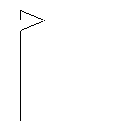
\includegraphics[width=3cm]{pics/fillpolygonsquare1.png}& 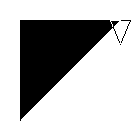
\includegraphics[width=3cm]{pics/fillpolygonsquare2.png}& 
\includegraphics[width=3cm]{pics/fillpolygonsquare3.png}& 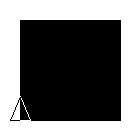
\includegraphics[width=3cm]{pics/fillpolygonsquare4.png}\\ 
			Passo 1& Passo 2& Passo 3& Passo 4\\
		\end{tabular}
	\end{center}
	\item Un secondo esempio che disegna e riempie una stella a cinque punte:\\
	\lstinline$Ripeti 5 [Av 100 RiempiPoligono [In 100 DX 144 Av 100 ] In 100 SX 72]$
	\begin{center}
		\begin{tabular}{ccccc}
			
\includegraphics[width=3cm]{pics/fillpolygon1.png}& 
\includegraphics[width=3cm]{pics/fillpolygon2.png}& 
\includegraphics[width=3cm]{pics/fillpolygon3.png}& 
\includegraphics[width=3cm]{pics/fillpolygon4.png}& 
\includegraphics[width=3cm]{pics/fillpolygon5.png}\\
			Passo 1& Passo 2& Passo 3& Passo 4&Passo 5\\
		\end{tabular}
	\end{center}
\end{itemize}



\section{Comandi di interruzione}
Un comando di interruzione può essere impiegato nel programma logo per terminare il programma stesso o una procedura o un ciclo. \xlogo\ ha tre comandi di interruzione: \texttt{Ferma}, \texttt{FermaTutto} e \texttt{Output}.\\
\label{break}

\prim{Ferma}{}
Interrompe l'esecuzione di una procedura o di un ciclo \texttt{Ripeti} o \texttt{Mentre} a seconda di dove lo si include.

\prim{FermaTutto}{} 
Il programma esce da tutte le procedure e si interrompe.\\

\prim{Output}{} 
Come \texttt{Ferma} interrompe una procedura ma, a differenza di questo, permette di restituire un valore.



\section{Modalità multitartaruga}
E' possibile avere più di una tartaruga attiva nell'area di disegno. Per impostazione predefinita, solo una tartaruga è disponibile. Per ``creare'' una nuova tartaruga si può usare la primitiva \texttt{ImpostaTartaruga} seguito dal numero di tartarughe voluto. Quando ci sono più tartarughe sull'area di disegno, solo una sarà quella attiva che risponderà ai comandi. Per prevenire ostacoli la tartaruga è creata all'origine ed è invisibile (occorre usare \texttt{MostraTartaruga} per visualizzarla). La nuova tartaruga è la tartaruga attiva, obbedisce a tutte le classiche primitive fino a ché non si cambierà la tartaruga attiva con \texttt{ImpostaTartaruga}. Il numero massimo di tartarughe può essere impostato nel Menu Strumenti$\to$Preferenze.\\
\\
Queste sono le primitive per la modalità multitartaruga:\\

\prim{ImpostaTartaruga, ImpTar}{n}
La tartaruga numero $n$ diventa la tartaruga attiva. Per impostazione predefinita la tartaruga attiva all'avvio di \xlogo\ è la numero 0, la sola visualizzata.\\

\prim{Tartaruga}{}
Restituisce il numero della tartaruga attiva. \\

\prim{Tartarughe}{}
Restituisce un elenco che contiene tutti i numeri delle tartarughe attualmente sull'area di disegno. \\

\prim{CancellaTartaruga, CancT}{n}
Elimina la tartaruga numero $n$.\\

\prim{ImpNumMaxT, ImpostaNumeroMassimoTartarughe}{n}
Imposta il numero massimo di tartarughe in modalità multitartaruga.\\

\prim{NumMaxT, NumMaxTartarughe}{}
Restituisce il numero massimo di tartarughe nella modalità multitartaruga.




\section{La tartaruga e le 3 dimensioni} \label{3D}
La tartaruga può lasciare il piano di disegno bidimensionale e spostarsi nelle 3 dimensioni. Per entrare nella modalità 3D si utilizza la primitiva \texttt{Prospettiva, 3D}. Benvenuti nel mondo 3D!
\subsection{La proiezione prospettica}
Per rappresentare lo spazio 3D su un piano 2D \xlogo\ utilizza la proiezione prospettica. Una cinepresa viene puntata alla scena 3D, dove l'immagine dallo schermo di proiezione viene visualizzata. Ecco un semplice schema esemplificativo: 
\begin{center}
	\includegraphics*[scale=0.6]{pics/perspective.png}
\end{center}
Alcune primitive permettono di impostare la posizione della cinepresa. Lo schermo di proiezione è posto a metà della distanza dalla cinepresa.

\subsection{Capire l'orientamento in un mondo 3D}
In un piano 2D l'orientamento della tartaruga è definito solo dalla sua direzione. In un mondo 3D l'orientamento della tartaruga è definito da 3 angoli:
\begin{itemize}
	\item Rollio: L'angolo della tartaruga attorno all'asse $(Oy)$
	\item Beccheggio: L'angolo della tartaruga attorno all'asse $(Ox)$
	\item Direzione: L'angolo della tartaruga attorno all'asse $(Oz)$ 
\end{itemize}
Nei fatti, per spostarsi in un mondo 3D, la tartaruga è molto simile ad un aereo. Di seguito una piccola illustrazione che rappresenta questi 3 valori:\\
\begin{minipage}{5.8cm}
	\begin{center}
		\includegraphics*[scale=0.3]{pics/plane-roll.png}
		\textbf{Rollio}
	\end{center}
\end{minipage}
\begin{minipage}{5.5cm}
	\begin{center}
		\includegraphics*[scale=0.35]{pics/plane-pitch.png}
		\textbf{Beccheggio}
	\end{center}
\end{minipage}
\begin{minipage}{5.5cm}
	\begin{center}
		\includegraphics*[scale=0.3]{pics/plane-heading.png}
		\textbf{Direzione}
	\end{center}
	\end{minipage}\\ \\
	Può sembrare un pò complesso all'inizio ma molti aspetti tendono ad essere molto simili allo spazio 2D. Queste sono le primitive di base per spostarsi in un mondo 3D:\\
	\prim{Avanti, Av, Indietro, In}{n}
	Stesso comportamento nel piano 2D e 3D.\\
	\prim{Destra, DX, Sinistra, SX}{n}
	Stesso comportamento nel piano 2D e 3D.\\
	\prim{RollioDestra, RDX}{n}
	La tartaruga ruota di $n$ gradi alla destra attorno al suo asse longitudinale.\\
	\prim{RollioSinistra, RSX}{n}
	La tartaruga ruota di $n$ gradi alla sinistra attorno al suo asse longitudinale.\\
	\prim{BeccheggiaSu, BeccheggiaSù, BS}{n}
	La tartaruga ruota di $n$ gradi in sù attorno al suo asse trasversale.\\
	\prim{BeccheggiaGiu, BeccheggiaGiù, BG}{n}
	La tartaruga ruota di $n$ gradi in giù attorno al suo asse trasversale. Nel piano bidimensionale, quando vogliamo disegnare un quadrato di latto 200, scriviamo \lstinline!Ripeti 4[Av 200 DX 90]!. Queste primitive sono disponibili nel mondo 3D dove il quadrato è disegnato in modalità prospettica. Se la tartaruga ruota in giù di $90$ gradi possiamo disegnare un altro quadrato e otteniamo: \\
	\begin{lstlisting}[caption="Due quadrati in 3D"]
	PulisciSchermo
	Ripeti 4[Av 200 DX 90] 
	BeccheggiaGiu 90
	Ripeti 4[Av 200 DX 90] 
	\end{lstlisting}
	\begin{minipage}{10cm}
		\begin{center}
			\includegraphics*[scale=0.4]{pics/perspective1.png}
		\end{center}
	\end{minipage}
	\\
	Occorre provare qualche esempio per capire questi angoli e diventare un esperto!\\
	Le tre primitive di rotazione sono collegate fra loro, per esempio si può provare il seguente codice:\\
	\begin{lstlisting}[caption="Movimento della tartaruga in 3D equivalente a \texttt{Sinistra~90}."]
	PulisciSchermo
	RollioSinistra 90 BeccheggiaSu 90 RollioDestra 90
	\end{lstlisting}


	\subsection{Primitive disponibili sia in modalità 2D sia in 3D}
	Le seguenti primitive sono disponibili nel piano bidimensionale e tridimensionale. La sola differenza risiede negli argomenti forniti alle primitive. Per esempio la primitiva \texttt{ImpostaPosizione} o \texttt{ImpPos} si aspetta un elenco come argomento ma, in modalità 3D, l'elenco deve contenere tre numeri $(x;y;z)$ che rappresentano le coordinate rispetto ai 3 assi. Questo è l'elenco di queste primitive:\\

\begin{center}
	\begin{tabular}{|cccc|}
		\hline
		\texttt{Cerchio, Circonferenza}&
		\texttt{Arco}&
		\texttt{Origine}&
		\texttt{Verso}\\
		\hline
		\texttt{Distanza}&
		\texttt{ImpPos, ImpostaPosizione}&
		\texttt{ImpX, ImpostaX}&
		\texttt{ImpY, ImpostaY}\\
		\hline
		\texttt{ImpDir, ImpostaDirezione}&
		\texttt{Etichetta}&
		\texttt{LunghezzaEtichetta, LE}&
		\texttt{Punto}\\
		\hline
		\texttt{Posizione, Pos}&
		\texttt{Direzione} & &\\
		\hline
	\end{tabular} \\ \vspace{0.5cm}
\end{center}

\subsection{Primitive disponibili solo in modalità 3D}

\prim{ImpostaXYZ, ImpXYZ}{x y z} 
Imposta la posizione della tartaruga nello spazio 3D. Accetta 3 argomenti ossia le coordinate x, y, z del punto desiderato. \texttt{ImpXYZ} è molto simile a \texttt{ImpPos} ma, a differenza di quest'ultimo, le coordinate non sono fornite come elenco. \\
Per esempio, \texttt{ImpXYX -100 200 50}: sposta la tartaruga al punto di coordinate $x=-100;y=200;z=50$\\
\prim{ImpZ}{z}
Sposta la tartaruga al punto con un valido valore $z$. \texttt{ImpZ} richiede un numero come argomento. Questa primitiva è analoga a \texttt{ImpX} e \texttt{ImpY}. \\
\prim{ImpostaOrientamento, ImpOr}{elenco}
Imposta l'orientamento della tartaruga. Questa primitiva accetta un elenco di tre elementi come argomento: angolo di rollio, di beccheggio e di direzione.\\
Per esempio, \texttt{ImpOr [100 0 58]}: la tartaruga ha rollio pari a 100 gradi, beccheggio pari a 0, direzione 58 gradi.\\
\prim{Orientamento}{}
Restituisce l'orientamento della tartaruga come un elenco che contiene \texttt{[~rollio~beccheggio~direzione~]}. Per esempio, se l'orientamento è \texttt{[100 20 90]}, significa che se si desidera replicare lo stesso orientamento dalla posizione originale (dopo un \texttt{PulisciSchermo}) occorrerà spostare la tartaruga come segue:
\begin{center}
	\texttt{ RDX 100 BS 20 DX 90}
\end{center}
Se si inverte l'ordine delle istruzioni, l'orientamento finale sarà diverso!\\
\prim{ImpostaRollio, ImpRol}{n} 
La tartaruga ruota attorno al suo asse longitudinale fino all'angolo fornito in argomento\\
\prim{Rollio}{}
Restituisce il valore corrente di rollio.\\
\prim{ImpostaBeccheggio, ImpBec}{n}
La tartaruga ruota attorno al suo asse trasversale fino all'angolo fornito in argomento.\\
\prim{Beccheggio}{}
Restituisce il valore corrente di beccheggio.
\subsection{Visualizzatore 3D}
\xlogo\ include un visualizzatore 3D, permette di visualizzare i disegni in 3D. Questo modulo utilizza la libreria Java3D che, quindi, è un requisito di installazione per un funzionamento appropriato di questa modalità.\\ \\
Il visualizzatore richiede l'osservanza di alcune regole:\\
quando si crea una figura geometrica nell'area di disegno occorre indicare al visualizzatore 3D quale forma si vuole disegnare per renderne possibile la futura visualizzazione. E' possibile disegnare poligoni (superfici), linee, punti, o testo. Per usare questa possibilità occorre utilizzare le seguenti primitive:\\ \\
\prim{InizioPoligono}{}
I successivi movimenti della tartaruga sono salvati per creare un poligono.\\
\prim{FinePoligono}{}
A partire dall'ultimo \texttt{InizioPoligono}, la tartaruga si è spostata attraverso numerosi vertici. Questo nuovo poligono è salvato, il suo colore è definito dal colore di tutti i vertici. Questa primitiva finalizza il poligono. \\
\prim{InizioLinea, IL}{}
I successivi movimenti della tartaruga sono salvati per creare una linea. \\
\prim{FineLinea, FL}{}
A partire dall'ultimo \texttt{InizioLinea}, la tartaruga si è spostata attraverso numerosi vertici. Questa nuova linea è salvata, il suo colore è definito dal colore di tutti i vertici. Questa primitiva finalizza la linea. \\
\prim{InizioPunto, IP}{} 
I successivi movimenti della tartaruga sono salvati per creare un set di punti. \\
\prim{FinePunto, FP}{}
Finalizza il set di punti.\\
\prim{InizioTesto, IT}{}
Ogni volta che si scrive del testo nell'area di disegno con la primitiva \texttt{Etichetta}, esso verrà salvato e quindi visualizzata dal visualizzatore 3D.\\
\prim{FineTesto, FT}{}
Fine della registrazione del testo.\\
\prim{VistaPoligono3D, VP3D}{}
Parte il visualizzatore 3D, tutti gli oggetti salvati sono disegnati in questa nuova finestra. Si ha il controllo della scena della cinepresa:
\begin{itemize}
	\item Si può ruotare la scena cliccando il testo sinistro del mouse.
	\item Si può traslare la scena cliccando il tasto destra del mouse.
	\item Si può ingrandire la scena con la rotella del mouse.
\end{itemize}
\subsection{Disegnare un cubo}
\noindent Tutte le facce sono quadrati di 400 passi. Questo è il programma:
\begin{lstlisting}[caption="Disegno di un cubo in 3D"]
Per quadrato
	# salviamo il quadrato verticale
	InizioPoligono Ripeti 4[Avanti 400 RuotaDestra 90] FinePoligono
Fine

Per SempliceCubo
	# cubo giallo
	PulisciSchermo 3D ImpostaColorePenna Giallo
	# facce laterali
	Ripeti 4[quadrato PennaSu RuotaDestra 90 Avanti 400 RuotaSinistra 90 
	RollioDestra 90 PennaGiu]
	# faccia inferiore
	BeccheggiaGiu 90 quadrato BeccheggiaSu 90
	# faccia superiore
	Avanti 400 BeccheggiaGiu 90 quadrato
	# visualizzazione
	VistaPoligono3D
Fine
\end{lstlisting}
Il programma si lancia con il comando: \texttt{SempliceCubo}:
\begin{center}
	\includegraphics*[scale=0.4]{pics/3dCube1.png}
\end{center}
Se sostituiamo nella procedura \texttt{quadrato}, \texttt{InizioPoligono} con \texttt{InizioLinea} e \texttt{FinePoligono} con \texttt{FineLinea}
\begin{center}
	\includegraphics*[scale=0.4]{pics/3dCube2.png}
\end{center}
Se si fosse utilizzata la primitiva \texttt{InizioPunto} e \texttt{FinePunto} invece di \texttt{InizioLinea} e \texttt{FineLinea}, si sarebbero visti su schermo solo gli otto vertici del cubo. Queste primitive sono molto utili per visualizzare il set di punti nello spazio 3D.


\subsection{Illuminare la scena}
Si possono impostare fino a quattro luci nella scena 3D. Come impostazione predefinita, la scena 3D ha solo due luci puntiformi abilitate. Cliccando su uno dei quattro bottoni delle luci nel modellizzatore 3D, la seguente finestra di dialogo comparirà:
\begin{center}
	\includegraphics*[scale=0.6]{pics/CaptureLight.png}
\end{center}
Sono disponibili svariati tipi di illuminazione:
\begin{itemize}
	\item Illuminazione di ambiente: è una luce uniforme, è possibile specificarne il colore.
	\item Illuminazione unidirezionale: si diffonde lungo una direzione costante. E' molto simile alla illuminazione puntuale quando la sorgente di luce è molto lontana dall'osservatore, come nel caso del sole, per esempio.
	\item Illuminazione puntiforme: la luce ha una posizione puntiforme, simile alle luci frontali.
	\item Illuminazione spot: è una luce puntiforme ma la luce è visualizzata come un cono di luce. Occorre specificare un valore angolare per il cono stesso.
\end{itemize}
La cosa migliore è giocare con le illuminazioni per capire come funzionano!


\subsection{Effetto nebbia}
Si può aggiungere un effetto di opacità alla scena 3D cliccando sul bottone nebbia nella scena 3D:
\begin{center}
	\includegraphics*[scale=0.6]{pics/CaptureFog.png}
\end{center}
Sono disponibili due tipi di nebbia:
\begin{itemize}
	\item Nebbia progressiva: l'opacità della nebbia è progressiva, occorre specificare due parametri:
	\begin{itemize}
		\item La distanza alla quale la nebbia inizia.
		\item La distanza alla quale l'opacità è completa.\\
	\end{itemize}
	\item Nebbia uniforme: questa nebbia è uniforme in tutta la scena. Occorre specificare la densità della nebbia.
\end{itemize}
\vspace*{0.2cm}
Esempio con nebbia progressiva:
\begin{center}
	\includegraphics*[scale=0.4]{pics/example-fog.png}
\end{center}



\section{Riprodurre musica}
\subsection{Riprodurre musica usando il sintetizzatore MIDI}
Per riprodurre musica MIDI occorre inserire lo spartito in un elenco di note (sequenza). Queste sono le regole da seguire per creare una sequenza valida:\\
\texttt{do re mi fa sol la si} : le classiche note della prima ottava.\\
Per riprodurre un re alto, scriviamo \texttt{re +}\\
Per riprodurre un re basso scriviamo \texttt{re -}\\
Se si vuole alzare o abbassare ottava, si usa il simbolo ``:'' seguito da ``+'' or ``-''. Per esempio: dopo ``:++'' nella sequenza, tutte le note saranno riprodotte due ottave sopra.\\
Per impostazione predefinita, le note sono riprodotte per la lunghezza di 1. Se si vuole aumentare o diminuire la durata occorre scrivere il numero che corrisponde alla durata delle note. Per esempio: \texttt{Seq [sol 0.5 la si]}. riprodurrà ``sol'' con una durata di 1 e ``la si'' con durata 0,5 (il doppio della velocità).\\


\prim{Sequenza, Seq}{elenco}
Pone in memoria la sequenza nell'elenco aggiungendola alle sequenze precedenti.\\

\prim{Suona}{}
Riproduce la sequenza in memoria. \\

\prim{ImpostaStrumento, ImpStr}{n}
Imposta lo strumento identificato da $n$. L'elenco di tutti gli strumenti disponibili si trova nel nel Menu Strumenti$\to$Preferenze$\to$Tab Suono.\\

\prim{Strumento}{}
Restituisce il numero che corrisponde allo strumento in uso. \\

\prim{ImpostaIndiceInSequenza, ImpSeq}{n}
Pone il cursore all'indice $n$ nella sequenza attuale in memoria.\\

\prim{IndiceSequenza, IndSeq}{}
Restituisce la posizione del cursore nella sequenza attiva.\\

\prim{CancellaSequenza, CancSeq}{}
Elimina la sequenza attiva in memoria. \\ 

Esempio di riproduzione MIDI:\\
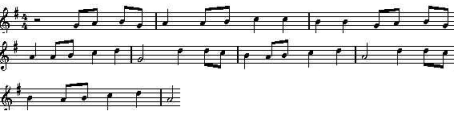
\includegraphics{pics/partition.png}
\begin{lstlisting}[caption="Creazione di uno spartito MIDI"]
Per tabac
# Crea la sequenza di note
seq [0.5 sol la si sol 1 la 0.5 la si 1 :+ do do :- si si 0.5 sol la si sol
          1 la 0.5 la si 1 :+ do re 2 :- sol ]
seq [:+ 1 re 0.5 re do 1 :- si 0.5 la si 1 :+ do re 2 :- la ]
seq [:+ 1 re 0.5 re do 1 :- si 0.5 la si 1 :+ do re 2 :- la ]
seq [0.5 sol la si sol 1 la 0.5 la si 1 :+ do do :- si si 0.5 sol la si sol
          1 la 0.5 la si 1 :+ do re 2 :- sol ]
Fine
\end{lstlisting}

Per ascoltare la musica, eseguire il comando: \texttt{tabac Suona}\\
Un altro esempio mostra una interessante applicazione della primitiva \texttt{ImpSeq}:\\
\begin{lstlisting}[caption="Riproduzione di uno spartito MIDI"]
CancSeq
tabac
ImpSeq 2
tabac
Suona
\end{lstlisting}



\subsection{Riprodurre file MP3}

\prim{Avviamp3}{parola1}
Legge e riproduce il file mp3 \textit{parola1}. Il file deve risiedere nella cartella attuale oppure può essere localizzato in rete. Per esempio:\\
\texttt{Avviamp3 file.mp3}\\
\texttt{Avviamp3 http://website.com/file.mp3}\\

\prim{Fermamp3}{}
Ferma la riproduzione del file mp3 attuale.






\section{Interagire con l'utente durante l'esecuzione del programma}
%At the moment, XLOGO can interact with the user during the execution
%of a program through the keyboard and through the mouse.

\subsection{Interazione tramite la tastiera}
Attualmente il testo può essere accettato dall'utente durante l'esecuzione del programma attraverso tre primitive:
\begin{enumerate}
	\item \texttt{Tasto?}
	\item \texttt{LeggiCarattere}
	\item \texttt{Leggi}
\end{enumerate}

\prim{Tasto?}{}
Restituisce ``vero'' o ``falso'' a seconda che l'utente abbia premuto un tasto dall'avvio del programma LOGO.\\

\prim{LeggiCarattere}{}
\begin{itemize}
	\item Se \texttt{Tasto?} è falso il programma viene messo in pausa fino a che l'utente preme un tasto.
	\item Se \texttt{Tasto?} è vero restituisce il codice unicode dell'ultimo tasto che è stato premuto.
\end{itemize}
E' opportuno ricordare che \texttt{LeggiCarattere} non ritorna il carattere ma il suo codice unicode, per convertirlo in carattere utilizzare la primitiva \texttt{Carattere} (vedi pagina \pageref{car}).
Questi sono il valori per alcuni tasti speciali:\\
\begin{table}[h]
	\begin{tabular}{|llll|}
		\hline
		Carattere & Codice unicode & Carattere & Codice unicode\\
		\hline
		$\leftarrow$	& -37 or -226 (NumPad)	& $\uparrow$	& -38 or -224 (NumPad)\\
		$\rightarrow$	& -39 or -227 (NumPad)	& $\downarrow$	& -40 or -225 (NumPad)\\
		ESC 			& 27 					& F1			& -112\\
		F2				& -113					& 				&\\
		Shift			& -16					& Spazio		& 32\\
		Ctrl			& -17					& Invio			& 10\\
		\hline
	\end{tabular}
	\caption{Caratteri e rispettivi codici unicode}
\end{table}
Se si è insicuri dal valore restituito da un tasto, si può digitare:\\
\texttt{Stampa LeggiCarattere}. L'interprete aspetterà la pressione di un tasto prima di fornire il valore corrispondente.\\
\\

\prim{Leggi}{elenco1 arg2}
Visualizza una finestra di dialogo il cui titolo è \textit{elenco1}. L'utente può quindi inserire una risposta in un campo di testo. La risposta sarà salvata nella forma di parola o elenco (se l'utente ha scritto più parole) nella variabile \textit{arg2}, che sarà assegnata quando il bottone OK viene premuto.

\subsection{Qualche esempio di utilizzo}

\begin{lstlisting}[caption="Richiesta di una risposta dall'utente"]
per vintage
	Leggi [Che eta' hai?] "age
	AssegnaVar "age :age
	Se :age<18 [Stampa [Sei minorenne]]
	Se o :age=18 :age>18 [Stampa [Sei un adulto]]
	Se :age>99 [Stampa [Rispetto e' dovuto!!]]
fine
\end{lstlisting}

\begin{lstlisting}[caption="L'utente controlla la tartaruga"]
per rallye
	Se Tasto? [
	  AssegnaVar "car LeggiCarattere
	  Se :car=-37 [RuotaSinistra 90]
	  Se :car=-39 [RuotaDestra 90]
	  Se :car=-38 [Avanti 10]
	  Se :car=-40 [Indietro 10]
	  Se :car=27 [FermaTutto]
	]
fine
\end{lstlisting}



\subsection{Interazione tramite il mouse}
Attualmente gli eventi del mouse possono essere accettati dall'utente durante l'esecuzione del programma attraverso tre primitive:
\begin{enumerate}
	\item \texttt{LeggiMouse}
	\item \texttt{PosizioneMouse}
	\item \texttt{Mouse?}
\end{enumerate}

\prim{LeggiMouse}{}
L'esecuzione del programma viene messa in pausa in attesa di un evento del mouse. Restituisce un numero che rappresenta l'evento avvenuto. I valori sono:
\begin{itemize}
 \item 0$\to$Il mouse è stato mosso.
 \item 1$\to$Il bottone 1 è stato premuto.
 \item 2$\to$Il bottone 2 è stato premuto.
\end{itemize}
Il bottone 1 è quello di sinistra, il bottone 2 è quello alla sua destra e così via \textellipsis\\

\prim{PosizioneMouse, PosMouse}{}
Restituisce un elenco contenente la posizione del mouse.\\

\prim{Mouse?}{}
Restituisce ``vero'' se si tocca il mouse dall'inizio del programma LOGO, ``falso'' altrimenti.



\subsection{Qualche esempio di utilizzo}

\begin{lstlisting}[caption="La tartaruga segue il mouse quando si sposta sullo schermo"]
Per esempio
	Se LeggiMouse=0 [ImpPos PosMouse]
Fine
RipetiPerSempre [esempio]
\end{lstlisting}

\begin{lstlisting}[caption="La tartaruga segue il mouse con il tasto premuto"]
Per esempio2
	if LeggiMouse=1 [ImpPos PosMouse]
Fine
RipetiPerSempre [esempio2]
\end{lstlisting}

In questo esempio si creano due bottoni rosa. Se si clicca sul bottone di sinistra viene disegnato un quadrato di lato 40, se si clicca sul bottone di destra viene disegnato un piccolo cerchio. Se si clicca il tasto destro sul bottone destro il programma viene fermato. Il programma si avvia con \texttt{avvio}:

\includegraphics*[width=15 cm]{pics/lissouris.png} 
\begin{lstlisting}[caption="Disegno di poligoni con il mouse"]
per bottone
	#crea un bottone rettangolare rosa 
	Ripeti 2[Avanti 50 RuotaDestra 90 Avanti 100 RuotaDestra 90] 
	RuotaDestra 45 PennaSu Avanti 10 PennaGiu ImpostaColorePenna [255 153 153]
	Riempi Indietro 10 RuotaSinistra 45 PennaGiu ImpostaColorePenna 0
fine

per avvio
	PulisciSchermo bottone PennaSu ImpostaPosizione [150 0] PennaGiu bottone
	PennaSu ImpostaPosizione [30 20] PennaGiu Etichetta "quadrato
	PennaSu ImpostaPosizione [180 20] PennaGiu Etichetta "cerchio
	PennaSu ImpostaPosizione [0 -100] PennaGiu
	mouse
fine

per mouse
	# assegniamo il valore di LeggiMouse nella variabile ev
	AssegnaVar "ev LeggiMouse
	# assegniamo la coordinata x del mouse nella variabile x
	AssegnaVar "x Elemento 1 PosizioneMouse
	# assegniamo la coordinata y del mouse nella variabile y
	AssegnaVar "y Elemento 2 PosizioneMouse
	# se si clicca sul bottone di sinistra
	Se :ev=1 & :x>0 & :x<100 & :y>0 & :y<50 [square]
	# se si clicca sul bottone di destra
	Se  :x>150 & :x<250 & :y>0 & :y<50 [
	          Se :ev=1 [Circonferenza2]
	          Se :ev=3 [Ferma]
	]
	mouse
fine

per Circonferenza2
	Circonferenza 20 PennaSu  Avanti 40 RuotaDestra 90 PennaGiu
fine

per square
	Ripeti 4 [Avanti 40 RuotaDestra 90] RuotaDestra 90 Avanti 40 RuotaSinistra 90
fine
\end{lstlisting} 


\subsection{Componenti grafici}
Con \xlogo\, si possono aggiungere molti componenti grafici nell'area di disegno (bottoni e menu). Tutte le primitive che permettono la manipolazione di queste componenti terminano con il suffisso \textsc{GUI} (per ``Graphical User Interface'' Interfaccia grafica con l'utente).\\
L'aggiunta di un componente segue tre passi:
\begin{enumerate}
	\item Creazione
	\item Modifica delle proprietà
	\item Visualizzazione sull'area di disegno
\end{enumerate}

\subsubsection{Creare un componente}

\prim{BottoneGUI, BGUI}{parola1 parola2}
Crea un bottone il cui titolo è \textit{parola2} ed il cui nome è \textit{parola1}. Il nome identifica il componente per i successivi passi. \\

\prim{MenuGUI, MGUI}{parola1 elenco2}
Crea un menu combinato il cui nome è \textit{parola1} e che contiene gli elementi da \textit{elenco2}\\
\texttt{MenuGUI "mioMenu [elemento1 elemento2 elemento3]}

\subsubsection{Modificare le proprietà del componente} 

\prim{PosizioneGUI, PGUI}{parola1 elenco2} 
Posiziona l'elemento grafico \textit{parola1} in un punto preciso fornito dalle coordinate in \texttt{elenco2}. Per esempio, volendo posizionare il bottone ``b'' alle coordinate $(20;100)$, si scriverà: \lstinline!PosizioneGUI "b [20 100]!. Se non si specifica una posizione per il componente, verrà posizionato nell'angolo in alto a sinistra dell'area di disegno.\\

\prim{RimuoviGUI, RGUI}{parola1}
Cancella un componente grafico. Per esempio per cancellare il bottone ``b'': \lstinline!lRimuoviGUI "b!.

\prim{AzioneGUI, AGUI}{parola1 elenco2}
Definisci una azione per il componente \texttt{parola1} quando l'utente interagisce con esso.\\
\begin{lstlisting}[caption="Esempi di \texttt{AzioneGUI}"]
# la tartaruga avanza di 100 passi se si clicca il bottone "b
AzioneGUI "b [fd 100 ]
# Nel menu combinato, ciascun elemento ha la sua azione
AzioneGUI "m [[Stampa "elemento1]  [Stampa "elemento2] [Stampa "elemento3]]
\end{lstlisting}
\noindent


\subsubsection{Modificare le proprietà del componente}
\prim{DisegnaGUI, DGUI}{parola1}
Visualizza il componente grafico nell'area di disegno. Per esempio per mostrare il bottone ``b'' \lstinline!DisegnaGUI "b!.



\section{Ora e data}
\xlogo\ ha numerose primitive per la data, l'ora e per generare conteggi inversi.\\

\prim{Aspetta}{n}
 Sospende l'esecuzione del programma e quindi la tartaruga per $\frac{n}{60}$ secondi. Per esempio per sospendere il programma per 1 secondo: \texttt{Aspetta 60}.  \\

\prim{Cronometro}{n}
Inizia un conteggio inverso di $n$ secondi. Il programma può controllare se il conteggio è terminato con  \texttt{FineCronometro?}\\

La differenza tra \texttt{Aspetta} e \texttt{Cronometro} rimane nel fatto che la seconda primitiva non sospende il programma.\\

\begin{lstlisting}[caption="Uso della primitiva \texttt{cronometro}"]
per orologio
	Se FineCronometro? [
		PulisciSchermo 
		ImpCFont NascondiTartaruga
		AssegnaVar "heu HMS
		AssegnaVar "h Primo :heu
		AssegnaVar "m Elemento 2 :heu
		Se :m-10<0 [AssegnaVar "m Parola 0 :m]
		AssegnaVar "s Ultimo :heu
		Se :s-10<0 [AssegnaVar "s Parola 0 :s]
		Etichetta Parola Parola Parola Parola :h ": :m ": :s 
		Cronometro 5
	]
fine
\end{lstlisting} 


\prim{FineCronometro?}{}
Restituisce \texttt{"vero} se non c'è un conteggio attivo, altrimenti restituisce \texttt{"falso}.\\

\prim{Data}{}
Restituisce un elenco contenente tre numeri interi rappresentanti la data di sistema. Il primo intero indica il giorno, il secondo il mese, il terzo l'anno ([giorno mese anno]).\\

\prim{HMS}{}
Restituisce un elenco di tre interi rappresentanti l'ora di sistema. Il primo intero identifica l'ora, il secondo i minuti, il terzo i secondi [ora minuto secondo]\\

\prim{SecondiDaAvvio}{}
Restituisce il tempo passato in secondi da quando \xlogo\ è stato lanciato.\\



\section{Utilizzare \xlogo\ in rete}
\label{network}

\subsection{Basi delle reti}
Introduciamo le basi della comunicazione in rete prima di utilizzare le primitive di \xlogo.
\begin{figure}[h]%
	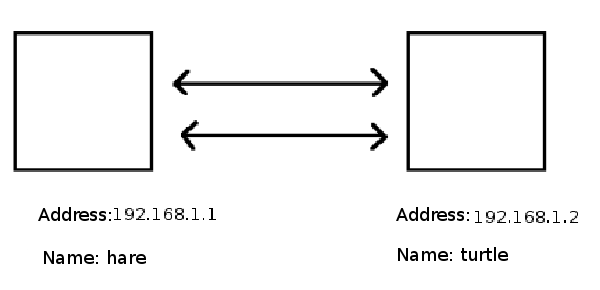
\includegraphics{pics/network.png}
	\caption{Una semplice rete}
\end{figure}

Due o più computer possono comunicare in rete se entrambi possiedono schede di rete Ethernet. Ciascun computer è identificato da un indirizzo univoco chiamato \textit{indirizzo~IP}. Questo indirizzo IP consiste di 4 numeri interi, ciascuno compreso tra 0 e 255 e separati da punti. Per esempio l'indirizzo IP del primo computer in figura è 192.168.1.1.\\
Poiché non è facile ricordare questi indirizzi è anche possibile identificare ciascun computer con un nome più semplice. Come possiamo vedere in figura, possiamo comunicare con il computer di destra attraverso il suo indirizzo IP 192.168.1.2 o tramite il suo nome: \texttt{turtle}\\
Il computer locale sul quale si lavora ha sempre uno stesso indirizzo IP: 127.0.0.1, il suo nome generale è texttt{localhost}. Lo vedremo in pratica più oltre.
 
\subsection{Primitive per la rete} 
\xlogo\ ha quattro primitive che gli consentono di comunicare in rete:
\begin{enumerate}
	\item \texttt{AscoltaTCP}
	\item \texttt{EseguiTCP}
	\item \texttt{FinestraChatTCP}
	\item \texttt{InviaTCP}
\end{enumerate} 
Nei successivi esempi si assume la configurazione dei due computer nella figura precedente.

\prim{AscoltaTCP, ATCP}{}
Questa primitiva è la base di tutta la comunicazione in rete. Non ha bisogno di un argomento. Il computer si dispone in ascolto delle istruzioni spedite da altri computer nella rete. \\

\prim{EseguiTCP, ETCP}{parola1 elenco2}
Questa primitiva permette l'esecuzione di istruzioni da un computer in rete. L'indirizzo IP del computer in rete è fornito in \textit{parola1}, l'elenco \textit{elenco2} contiene le istruzioni da eseguire.\\
Per esempio: mi trovo sul computer \texttt{hare}, voglio disegnare un quadrato di lato 100 sull'altro computer. Quindi sul computer \texttt{turtle}, devo lanciare la primitiva \texttt{listentcp}. Quindi sul computer \texttt{hare}, scrivo:\\
\begin{lstlisting}[caption="Disegno su un computer in rete"]
EseguiTCP "192.168.1.2 [ripeti 4[avanti 100 ruotadestra 90]]
# o 
EseguiTCP "turtle [ripeti 4[avanti 100 ruotadestra 90]]
\end{lstlisting} 

\prim{FinestraChatTCP, FChatTCP}{parola1 elenco2}
Permette una chat tra due computer in rete. Su ciascun computer viene visualizzata una finestra di chat. \textit{parola1} è l'indirizzo IP del computer o il suo nome, \textit{elenco2} contiene la frase da visualizzare.\\
Per esempio: \texttt{hare} vuole parlare con \texttt{turtle}.\\
Per prima cosa \texttt{turtle} esegue \texttt{AscoltaTCP}, in questo modo rimane in attesa di istruzioni da computer in rete. Quindi \texttt{hare} scrive: \texttt{FinestraChatTCP~\textquotedbl 192.168.1.2~[ciao turtle]}.\\
Le finestre chat compariranno su entrambi i computer, permettendogli di parlare fra di loro.\\ 

\prim{InviaTCP, ITCP}{parola1 elenco2}
Spedisce dati verso un computer in rete e restituisce la sua risposta. \textit{parola1} è l'indirizzo IP del computer o il suo nome, \textit{elenco2} contiene i dati da spedire. Quando \xlogo\ è lanciato sull'altro computer, risponderà OK. E' possibile comunicare con un robot attraverso la sua interfaccia di rete. La risposta del robot potrebbe quindi variare. \\
Per esempio: \texttt{turtle} vuole spedire a \texttt{hare} la frase ``3.14159 è una approssimazione di pi greco''.\\
\texttt{hare} esegue \texttt{AscoltaTCP}. \texttt{turtle} scrive: \texttt{Stampa~InviaTCP~\textquotedbl hare~[3.14159 è una approssimazione di pi greco]}.\\ \\
\textbf{Un piccolo suggerimenti}: Apri due volte \xlogo\ sullo stesso computer.
\begin{itemize}
	\item Nella prima finestra, esegui \texttt{AscoltaTCP}.
	\item Nella seconda finestra, scrivi \texttt{EseguiTCP \textquotedbl 127.0.0.1 [avanti 100 ruotadestra 90]}
\end{itemize}
Puoi muovere la tartaruga nell'altra finestra! Ciò è possibile perché 127.0.0.1 designa l'indirizzo locale, è quindi lo stesso computer \textellipsis




